\documentclass[12pt, a4paper]{article}

\usepackage{amssymb,amsmath,amsfonts,eurosym,geometry,ulem,graphicx,caption, xcolor,setspace,sectsty,comment,footmisc,caption,natbib,pdflscape,array,hyperref, fancyhdr, csquotes, tikz, enumitem, dsfont, amsthm, makecell, multicol,multirow, booktabs,xcolor,subcaption}

\usepackage{etex,etoolbox}
\usepackage{thmtools}
\usepackage[many]{tcolorbox}
\usepackage{apxproof}
\usepackage{listings}

\usepackage{tabularray}
\usepackage{float}
\usepackage{graphicx}
\usepackage{codehigh}
\usepackage[normalem]{ulem}
\UseTblrLibrary{booktabs}
\UseTblrLibrary{siunitx}
\newcommand{\tinytableTabularrayUnderline}[1]{\underline{#1}}
\newcommand{\tinytableTabularrayStrikeout}[1]{\sout{#1}}
\NewTableCommand{\tinytableDefineColor}[3]{\definecolor{#1}{#2}{#3}}


\usetikzlibrary{decorations.pathreplacing,positioning, arrows.meta}
\hypersetup{
    colorlinks=true,
    linkcolor=purple,
    filecolor=magenta,      
    urlcolor=purple,
    citecolor=purple,
    pdftitle={Overleaf Example},
    pdfpagemode=FullScreen,
    }
\normalem



\onehalfspacing
\newtheorem{theorem}{Theorem}[section]
\newtheorem{corollary}{Corollary}[theorem]
\newtheorem{lemma}[theorem]{Lemma}
\newtheorem{definition}{Definition}[section]
\newtheorem{remark}{Remark}
\newtheorem{assumption}{Hipótese}[section]
\newtheorem{proposition}{Proposition}[section]
\newtheoremrep{claim}{\sc \large Claim}[section]


\newtheorem{hyp}{Hypothesis}
\newtheorem{subhyp}{Hypothesis}[hyp]
\renewcommand{\thesubhyp}{\thehyp\alph{subhyp}}

\newtheorem{thm}{Hypothesis}[subsection]
\renewcommand{\thethm}{\Alph{subsection}.\arabic{thm}}


\newtheorem{inner}{\innerheader}
\newcommand{\innerheader}{}
\newenvironment{hypothesis}[1]
 {\renewcommand\innerheader{#1}\begin{inner}}
 {\end{inner}}

 \renewcommand{\refname}{\sc References}

\newcommand{\red}[1]{{\color{red} #1}}
\newcommand{\blue}[1]{{\color{blue} #1}}
\newcommand{\ImageWidth}{11cm}

\newcolumntype{L}[1]{>{\raggedright\let\newline\\arraybackslash\hspace{0pt}}m{#1}}
\newcolumntype{C}[1]{>{\centering\let\newline\\arraybackslash\hspace{0pt}}m{#1}}
\newcolumntype{R}[1]{>{\raggedleft\let\newline\\arraybackslash\hspace{0pt}}m{#1}}

\geometry{left=1.0in,right=1.0in,top=1.0in,bottom=1.0in}

\title{\sc Guia de Pareamento}
\author{}
\date{}

\renewcommand*\contentsname{\sc Sumário}

\numberwithin{equation}{section}
\numberwithin{table}{section}
\numberwithin{figure}{section}

\newtcolorbox{boxH}{
    colback = sub, 
    colframe = main, 
    boxrule = 0pt, 
    leftrule = 0pt, % left rule weight
    breakable
}

\definecolor{codegreen}{rgb}{0,0.6,0}
\definecolor{codegray}{rgb}{0.5,0.5,0.5}
\definecolor{codepurple}{rgb}{0.1,0.2,0.5}
\definecolor{backcolour}{rgb}{0.95,0.95,0.92}

\lstdefinestyle{mystyle}{
    language = R,
    commentstyle=\color{codegray},
    keywordstyle=\color{codepurple},
    numberstyle=\tiny\color{codegray},
    stringstyle=\color{codepurple},
    basicstyle=\ttfamily\footnotesize,
    breakatwhitespace=false,         
    breaklines=true,                 
    captionpos=b,                    
    keepspaces=true,                 
    numbers=false,                    
    numbersep=5pt,                  
    showspaces=false,                
    showstringspaces=false,
    showtabs=false,                  
    tabsize=2,
    inputencoding=utf8,
    extendedchars=true,
    literate={á}{{\'a}}1 {ã}{{\~a}}1 {é}{{\'e}}1 {í}{{\'i}}1 {â}{{\^a}}1 {ó}{{\'o}}1 {ç}{{\c{c}}}1 {õ}{{\~o}}1 {à}{{\`a}}1
}

\lstset{style=mystyle}

\begin{document}

\maketitle
\tableofcontents
\pagebreak \newpage

\doublespacing


\section{\sc Introdução} \label{introducao}


\input{Sections/1 - Introdução}

\section{\sc Causalidade}\label{poder}

Antes de introduzirmos o pareamento, é necessário discutir a causalidade de maneira mais formal. Esta seção tem como objetivo fixar a notação básica, definir os principais estimandos de interesse e explicitar o problema do viés de seleção que surge na ausência de um desenho experimental.Para tanto, utilizaremos um exemplo real de política de treinamento, que acompanhará o restante do guia.

Iniciaremos o exemplo relacionando o programa ao modelo de resultados potenciais, em seguida discutiremos o caso sob uma ótica experimental e, por fim, mostraremos como essas mesmas ideias se estendem a contextos não experimentais, preparando o terreno conceitual para a introdução do pareamento.

\subsection{Avaliando um Programa de Treinamento}

O \textit{National Supported Work Demonstration} (NSW) foi um programa de treinamento profissional conduzido nos Estados Unidos na metade da década de 1970 pela \textit{Manpower Demonstration Research Corporation} (MDRC). O objetivo principal do NSW era ajudar trabalhadores em situação de vulnerabilidade, que tinham pouca experiência ou qualificações, a se inserir no mercado de trabalho. O programa oferecia emprego temporário, treinamento e acompanhamento psicológico dentro de um ambiente protegido — ou seja, uma espécie de “fase de transição” entre o desemprego e o mercado formal.

Os participantes selecionados recebiam emprego garantido por 9 a 18 meses, dependendo do grupo e da localidade. Trabalhavam em equipes pequenas, de três a cinco pessoas, e se reuniam regularmente com um conselheiro do programa para discutir dificuldades e desempenho. O trabalho era remunerado, embora com salários inferiores aos de empregos regulares, mas havia possibilidade de aumento conforme o desempenho e a assiduidade. Após o término do contrato, os participantes precisavam buscar trabalho no mercado comum — o NSW era, portanto, uma ponte temporária para o emprego formal. As atividades variavam: alguns trabalhavam em postos de gasolina, outros em gráficas ou oficinas, e homens e mulheres frequentemente exerciam funções diferentes.


Para avaliar o impacto do programa, a MDRC coletou dados sobre renda e características demográficas dos participantes e do grupo de controle no período inicial e em até quatro entrevistas de acompanhamento realizadas a cada nove meses.
Esses dados serviram para medir como o programa influenciava o emprego e a renda ao longo do tempo — sendo um dos primeiros experimentos sociais randomizados em políticas de emprego e uma referência clássica em avaliação de impacto.

Antes de entrarmos no assunto da causalidade, vamos baixar os dados desse experimento. Ao longo desse guia, utilizaremos o \textit{software} \texttt{R} para manipular os dados e estimar os resultados. Vamos começar limpando o ambiente do \texttt{R} e carregando os pacotes necessários.

\begin{boxH}
\begin{lstlisting}[language = R]
# Limpar o ambiente 
rm(list=ls())

library(tidyverse) # Manipulação de dados + gráficos
library(haven) # Abre diversos tipos de arquivos

# Estimações
library(sandwich)
library(lmtest)
library(car)
library(estimatr)

# Visualização
library(modelsummary)
library(kableExtra)
\end{lstlisting}
\end{boxH}

Agora, para baixarmos os dados, vamos criar uma função que acessa a pasta do GitHub em que os dados estão armazenados e, ao rodarmos essa função em que o argumento é o nome da base, os dados serão abertos no \texttt{R}.

\begin{boxH}
\begin{lstlisting}[language = R]
baixar_dados <- function(dados)
{
  link <- paste("https://github.com/scunning1975/mixtape/raw/master/", 
                     dados, sep = "")
  df <- read_dta(link)
  return(link)
}

nsw <- baixar_dados("nsw_mixtape.dta")
\end{lstlisting}
\end{boxH}

Por fim, iremos criar algumas variáveis que iremos utilizar em análises mais a frente.

\begin{boxH}
\begin{lstlisting}[language = R]
nsw <- nsw %>% 
    mutate(agesq = age^2, # Idade ao quadrado
           agecube = age^3, # Idade ao cubo
           educsq = educ^2, # Educação ao quadrado
           u74 = case_when(re74 == 0 ~ 1, TRUE ~ 0), # Desemprego 1974
           u75 = case_when(re75 == 0 ~ 1, TRUE ~ 0), # Desemprego 1975
           re74sq = re74^2, # Renda 1974
           re75sq = re75^2) # Renda 1975
\end{lstlisting}
\end{boxH}

\subsection{Resultados Potenciais}\label{po}

A avaliação do programa NSW tem como objetivo principal estimar os efeitos da participação no programa sobre os ganhos monetários reais dos participantes. Seguindo a lógica de \cite{ImbensRubin2015}, para cada indivíduo $i = 1,\dots,N$, definimos os resultados potenciais:

\begin{itemize}
    \item $Y_i(1)$ é o ganho monetário real do indivíduo $i$ caso ele participe do programa;
    \item $Y_i(0)$ é o ganho monetário real do indivíduo $i$ caso ele \textbf{não} participe do programa.
\end{itemize}

Assim, é possível definir o efeito causal do programa NSW \textbf{para cada indivíduo $i$}:
$$ \delta_i = Y_i(1) - Y_i(0)$$

Esse parâmetro captura a diferença entre os ganhos monetários reais que um indivíduo teria caso participasse do programa e aqueles que teria caso não participasse. No entanto, para cada indivíduo, apenas um desses resultados potenciais é observado em um dado período. Seja $D_i = 1$ caso o indivíduo $i$ tenha participado do programa e $D_i = 0$ caso contrário, o resultado observado pode ser escrito como:

$$
Y_i = D_i Y_i(1) + (1 - D_i) Y_i(0)
$$

Ou seja, se o indivíduo $i$ participou do programa, $D_i = 1$, então o ganho monetário real observado para esse indivíduo será $Y_i = Y_i(1)$. Caso ele não tenha participado do programa, $D_i = 0$, o ganho monetário real observado será $Y_i = Y_i(0)$.

Como não é possível comparar os resultados de ter participado do programa com os resultados de não ter participado do programa para um mesmo indivíduo, tentaremos comparar os indivíduos que participaram do programa com os indivíduos que não participaram do programa. Nosso objetivo é tentar estimar o efeito médio do tratamento (\textit{Average Treatment Effect} - ATE), ou o efeito médio do tratamento nos tratados (\textit{Average Treatment Effect on the Treated} - ATT), definidos por
$$
ATE = \mathbb{E}[Y_i(1) - Y_i(0)], \qquad ATT = \mathbb{E}[Y_i(1) - Y_i(0) \mid D_i = 1]
$$

\textbf{Será que conseguimos recuperar o ATE ou o ATT apenas comparando a média do grupo de tratamento com a média do grupo de controle?} 

Para respondermos essa pergunta, temos pensar no que observamos. Se observássemos todos os indivíduos, o valor esperado dos ganhos monetários reais dos indivíduos que participaram do programa NSW seria $\mathbb{E}[Y_i \mid D_i = 1]$. Para os indivíduos que não participaram do programa, o valor esperado seria $\mathbb{E}[Y_i \mid D_i = 0]$. Comparando os dois, temos que

\begin{equation}\label{viesselecao}
    \begin{split}
        \mathbb{E}[Y_i \mid D_i = 1] - \mathbb{E}[Y_i \mid D_i = 0] & = \mathbb{E}[Y_i(1) \mid D_i = 1] - \mathbb{E}[Y_i(0) \mid D_i = 0]\\
        & = \underbrace{\mathbb{E}[Y_i(1) \mid D_i = 1] \color{red} -\mathbb{E}[Y_i(0) \mid D_i = 1]\color{black}}_{\text{ATT}} \\
        & - \underbrace{\mathbb{E}[Y_i(0) \mid D_i = 0] \color{red} + \mathbb{E}[Y_i(0) \mid D_i = 1] \color{black}}_{\text{Viés de Seleção}}
    \end{split}
\end{equation}

\noindent onde a primeira igualdade vem da definição do resultado observado e a segunda igualdade vem do fato de que $\mathbb{E}[Y_i(0) \mid D_i = 1] - \mathbb{E}[Y_i(0) \mid D_i = 1] = 0$. 

A Equação \eqref{viesselecao} nos mostra que a resposta é não — pelo menos por enquanto. Na ausência de uma hipótese explícita sobre o processo de alocação do programa NSW, a simples comparação de médias entre o grupo de tratamento e o grupo de controle estará potencialmente viesada. O viés de seleção, definido como $\mathbb{E}[Y_i(0) \mid D_i = 1] - \mathbb{E}[Y_i(0) \mid D_i = 0]$, reflete a presença de características individuais que influenciam simultaneamente a decisão de participar do programa e os ganhos monetários potenciais.


Imagine, por exemplo, que a divulgação do programa NSW tenha atingido majoritariamente pessoas de maior escolaridade. Assim, acreditamos que a probabilidade de alguém ser tratado aumenta caso a escolaridade dessa pessoas for maior. Ainda, pessoas com maior escolaridade tendem a ter ganhos monetários maiores. Podemos visualizar as direções da causalidade no grafo abaixo:

\[
\begin{array}{ccccc}
  & & \text{Escolaridade} & & \\
  & \swarrow & & \searrow \\
  D & &\longrightarrow && Y
\end{array}
\]

Neste caso, ao compararmos o grupo de que participou do NSW com o grupo que não participou, estamos essencialmente comparando os ganhos monetários de pessoas com maior escolaridade com ganhos monetários de pessoas com menor escolaridade. Se acreditarmos que os ganhos monetários desses dois grupos é diferente, o que é totalmente plausível, então $\mathbb{E}[Y_i(0) \mid D_i = 1] - \mathbb{E}[Y_i(0) \mid D_i = 0] \neq 0$, ou seja, existe viés de seleção.

\subsection{Experimentos}

O diferencial do NSW é que ele foi um experimento aleatorizado: entre os candidatos elegíveis, alguns foram escolhidos aleatoriamente para participar, enquanto outros não foram selecionados e serviram como grupo de controle. Isso permitia avaliar de forma rigorosa o efeito causal do programa sobre a renda e o emprego dos participantes.

A aleatorização nos garante que a alocação do tratamento não depende de nenhuma característica individual. Em termos matemáticos, nós temos que
$$(Y_i(1), Y_i(0)) \perp D_i,$$

\noindent ou seja, participar ou não do programa é independente dos ganhos monetários potenciais. Isso significa que, ao compararmos as pessoas que participaram do NSW com as pessoas que não participaram, estaremos comparando pessoas com características semelhantes. Em média, a única coisa que difere um grupo do outro é a participação no programa. 

Na prática, não conseguimos verificar diretamente essa independência a partir dos dados. No entanto, em um experimento aleatorizado, ela é garantida pelo desenho do estudo, e não pelos dados em si. O que podemos fazer empiricamente é avaliar se os grupos de tratamento e controle são semelhantes em termos de suas características \textbf{observáveis}, $X_i$. Esse procedimento é conhecido como \textbf{análise de balanceamento} e tem caráter diagnóstico: ele fornece evidência indireta de que a aleatorização produziu grupos comparáveis, mas não a testa formalmente. Na prática, iremos verificar se a média das variáveis observáveis no grupo tratado é estatisticamente igual à média no grupo de controle, isto é, $\overline{X}_{D_i=1} = \overline{X}_{D_i=0}$. No \texttt{R}, utilizaremos o pacote \texttt{vtable} para produzir uma \textbf{tabela de balanceamento}.


\begin{boxH}
\begin{lstlisting}[language = R]
library(vtable)

nsw %>% select(c("treat","age", "educ","nodegree","marr", "black","hisp","re74","re75","u74","u75")) %>%
  sumtable(group = "treat", group.test=TRUE, digits = 3)
\end{lstlisting}
\end{boxH}

O código acima produz a Tabela \ref{balance}. Nela, temos dez características observáveis disponíveis. Para cada característica, temos a média e o desvio padrão para o grupo de tratamento e o grupo de controle, além do teste F de signifiância conjunta. Nela, podemos ver que as características estão, em geral, balanceadas. Apenas ensino médio incompleto tem uma diferença estatisticamente significante. Mesmo com a alocação do tratamento ter sido aleatória, podemos ter diferenças como essa devido ao baixo número de observações.

\begin{table}[!htbp] \centering \caption{Balanceamento}\label{balance}
\begin{tabular}{lccccccl}
\toprule
Tratamento & \multicolumn{3}{c}{0} & \multicolumn{3}{c}{1} &   \\
  \midrule
 Variável & \multicolumn{1}{c}{N} & \multicolumn{1}{c}{Média} & \multicolumn{1}{c}{SD} & \multicolumn{1}{c}{N} & \multicolumn{1}{c}{Média} & \multicolumn{1}{c}{SD} & \multicolumn{1}{c}{Teste F} \\ 
\midrule
Idade \hspace{70mm}& 260 & 25.1 & 7.06 & 185 & 25.8 & 7.16 & F$=1.247^{}$ \\ 
Educação & 260 & 10.1 & 1.61 & 185 & 10.3 & 2.01 & F$=2.237^{}$ \\ 
Ensino Médio Incompleto & 260 & 0.835 & 0.372 & 185 & 0.708 & 0.456 & F$=10.338^{***}$ \\ 
Pardo & 260 & 0.154 & 0.361 & 185 & 0.189 & 0.393 & F$=0.961^{}$ \\ 
Negro & 260 & 0.827 & 0.379 & 185 & 0.843 & 0.365 & F$=0.207^{}$ \\ 
Hispânico & 260 & 0.108 & 0.311 & 185 & 0.0595 & 0.237 & F$=3.153^{*}$ \\ 
Renda 1974 & 260 & 2107 & 5688 & 185 & 2096 & 4887 & F$=0^{}$ \\ 
Renda 1975 & 260 & 1267 & 3103 & 185 & 1532 & 3219 & F$=0.765^{}$ \\ 
Desemprego 1974 & 260 & 0.75 & 0.434 & 185 & 0.708 & 0.456 & F$=0.966^{}$ \\ 
Desemprego 1975 & 260 & 0.685 & 0.466 & 185 & 0.6 & 0.491 & F$=3.41^{*}$\\ 
\midrule
\multicolumn{8}{l}{Significância estatística: * $p<0.1$; ** $p<0.05$; *** $p<0.01$}\\ 
\end{tabular}

\end{table}

O ponto central da Tabela \ref{balance} é gerarmos evidência de que a alocação do tratamento não está correlacionada com nenhuma característica observada. Um bom balanceamento adicionado ao fato de a alocação do tratamento ter sido aleatorizada são ótimos passos para argumentar que um efeito causal está sendo recuperado na hora de estimar os resultados. Se estamos comparando dois grupos iguais em média, isso significa que $\mathbb{E}[Y_i(0) \mid D_i = 1] = \mathbb{E}[Y_i(0) \mid D_i = 0]$. Ou seja, agora o viés de seleção deixa de existir, e nossa comparação de médias é igual ao ATT:
$$
\mathbb{E}[Y_i \mid D_i = 1] - \mathbb{E}[Y_i \mid D_i = 0] = \mathbb{E}[Y_i(1) \mid D_i = 1]  -\mathbb{E}[Y_i(0) \mid D_i = 1] = ATT
$$

Como cada um dos resultados potenciais vão ser, em média, iguais para os grupos de tratamento e controle, isto é, $\mathbb{E}[Y_i(1) \mid D_i] = \mathbb{E}[Y_i(1)]$ e $\mathbb{E}[Y_i(0) \mid D_i] = \mathbb{E}[Y_i(0)]$, então a comparação de média entre os dois grupos não só retorna o ATT, como também o ATE:
$$
\mathbb{E}[Y_i \mid D_i = 1] - \mathbb{E}[Y_i \mid D_i = 0] = \mathbb{E}[Y_i(1) - Y_i(0)]  = ATE
$$

Podemos estimar esses parâmetros causais de duas maneiras: fazendo uma diferença de médias simples ou regredindo os ganhos monetários em participação no programa. A diferença de médias, nesse caso, é equivalente ao parâmetro de Mínimos Quadrados Ordinários (MQO) relacionado à variável de tratamento.\footnote{Apêndice} Aqui, iremos estimar esses efeitos através da seguinte regressão:
$$
Y_i = \alpha + \beta D_i + \varepsilon_i,
$$

\noindent em que $\varepsilon_i$ é o erro idiossincrático. Neste caso, o estimador de $\beta$, que iremos chamar de $\hat{\beta}$, irá recuperar o ATE. No \texttt{R}, iremos utilizar a função \texttt{lm\_robust} do pacote \texttt{estimatr} para rodarmos a regressão.

\begin{boxH}
\begin{lstlisting}[language = R]
# Igual à diferença de médias
fit_nsw = lm_robust(re78 ~ treat, se_type = "stata", data = nsw)

# Resultados
summary(fit_nsw)
\end{lstlisting}
\end{boxH}

A Tabela \ref{reg1} mostra os resultados da regressão. Ela nos diz que o programa NSW \textbf{causou}, em média, um aumento de \$1.794,342 aos participantes do programa.

\begin{table}[h]

\centering
\caption{Resultados da Regressão}
\begin{talltblr}[         %% tabularray outer open
entry=none,label=none,
note{}={+ p \num{< 0.1}, * p \num{< 0.05}, ** p \num{< 0.01}, *** p \num{< 0.001}},
]                     %% tabularray outer close
{                     %% tabularray inner open
colspec={Q[]Q[]},
column{2}={}{halign=c,},
column{1}={}{halign=l,},
hline{6}={1-2}{solid, black, 0.05em},
}                     %% tabularray inner close
\toprule
& Estimativa \\ \midrule %% TinyTableHeader
Intercepto \hspace{80mm} & \num{4554.801}*** \\
& (\num{340.204}) \\
Tratamento & \num{1794.342}** \\
& (\num{670.824}) \\
Observações & \num{445} \\
\bottomrule
\end{talltblr}\label{reg1}
\end{table} 

\subsection{Dados Não-Experimentais}

Até aqui, utilizamos o programa NSW como um exemplo ideal de avaliação causal, pois ele foi implementado como um experimento aleatorizado. A aleatorização garantiu que, em média, tratados e controles fossem comparáveis antes da intervenção, o que nos permitiu interpretar diretamente a diferença de médias como um efeito causal. No entanto, esse tipo de desenho é a exceção, e não a regra, na avaliação de políticas públicas. Na grande maioria das situações, o pesquisador dispõe apenas de dados observacionais, isto é, dados gerados sem qualquer controle direto sobre o processo de seleção para o tratamento.

Para ilustrar esse cenário, vamos agora considerar uma base de dados não-experimental: a \textit{Current Population Survey} (CPS), uma pesquisa domiciliar representativa da população dos Estados Unidos. Diferentemente do NSW, a CPS não foi desenhada para avaliar um programa específico. Ela contém informações sobre renda, escolaridade, idade, raça, entre outras características, mas a participação em programas de treinamento não é resultado de sorteio, e sim de decisões individuais, institucionais e sociais. Como consequência, ao compararmos indivíduos tratados e não tratados nesse contexto, estamos comparando grupos que podem ser estruturalmente muito diferentes entre si. Essa simples comparação não permite isolar o efeito causal do programa, pois está sujeita a viés de seleção: indivíduos que participam do treinamento podem diferir sistematicamente dos não participantes em características observadas e não observadas que também afetam os resultados.

Agora, vamos baixar os dados da CPS no \texttt{R} e juntar com os tratados da base anterior do NSW. A ideia é mostrar que, utilizando os indivíduos da base da CPS como controle, não teremos um grupo de comparação válido como o que tínhamos na nossa base experimental.

\begin{boxH}
\begin{lstlisting}[language = R]
# Baixar dados não-experimentais
cps <- baixar_dados("cps_mixtape.dta") 

# Juntar dados não-experimentais com o grupo tratado do experimento
nsw_treat <- nsw %>% filter(treat==1)

# Adicionar variáveis quadráticas e dummies
cps <- cps %>% 
  bind_rows(nsw_treat) %>% 
  mutate(agesq = age^2,
         agecube = age^3,
         educsq = educ*educ,
         u74 = case_when(re74 == 0 ~ 1, TRUE ~ 0),
         u75 = case_when(re75 == 0 ~ 1, TRUE ~ 0),
         re74sq = re74^2,
         re75sq = re75^2)
\end{lstlisting}
\end{boxH}

Após preparar os dados, iremos rodar a regressão usando os dados da CPS como controles. 

\begin{boxH}
\begin{lstlisting}[language = R]
# Diferença simples entre tratados e controle não-experimental
fit_nswcps = lm_robust(re78 ~ treat, se_type = "stata", data = cps)

modelsummary(fit_nswcps, stars = TRUE, fmt = 3, output = "latex")
\end{lstlisting}
\end{boxH}

A comparação entre os resultados da Tabela \ref{reg2}, baseada em dados não experimentais, e da Tabela \ref{reg1}, que utiliza a amostra experimental, ilustra de forma clara o problema do viés de seleção. Enquanto a regressão com dados experimentais aponta um efeito positivo e estatisticamente significativo do tratamento, refletindo o impacto causal médio estimado a partir de um desenho aleatório, a regressão com dados não experimentais produz uma estimativa fortemente negativa para o coeficiente do tratamento. Essa reversão de sinal não decorre de um efeito causal adverso do programa, mas sim do fato de que, na amostra não experimental, os indivíduos tratados diferem sistematicamente dos controles em características relevantes que também afetam o resultado. Em particular, participantes do programa tendem a apresentar piores condições iniciais no mercado de trabalho, o que gera uma correlação negativa espúria entre tratamento e desfecho quando essas diferenças não são adequadamente controladas. Esse contraste evidencia que, na ausência de aleatorização, estimativas ingênuas baseadas em regressões simples podem estar severamente enviesadas.

\begin{table}[h]
\centering
\caption{Resultados da Regressão com Dados Não-Experimentais}
\begin{talltblr}[         %% tabularray outer open
entry=none,label=none,
note{}={+ p \num{< 0.1}, * p \num{< 0.05}, ** p \num{< 0.01}, *** p \num{< 0.001}},
]                     %% tabularray outer close
{                     %% tabularray inner open
colspec={Q[]Q[]},
column{2}={}{halign=c,},
column{1}={}{halign=l,},
hline{6}={1-2}{solid, black, 0.05em},
}                     %% tabularray inner close
\toprule
& Estimativa \\ \midrule %% TinyTableHeader
Intercepto \hspace{80mm} & \num{14846.660}*** \\
& (\num{76.291}) \\
Tratamento & \num{-8497.516}*** \\
& (\num{581.916}) \\
Observações & \num{16177} \\
\bottomrule
\end{talltblr}\label{reg2}
\end{table} 

Esse contraste muda completamente a natureza do problema. Enquanto no experimento a igualdade entre grupos era garantida pelo desenho, nos dados não-experimentais essa igualdade precisa ser construída estatisticamente. Caso contrário, qualquer comparação direta entre tratados e não tratados estará contaminada por viés de seleção. Em termos do modelo de resultados potenciais discutido na Seção \ref{po}, o problema central é que, sem um experimento, não conseguimos garantir que
$$
\mathbb{E}[Y_i(0) \mid D_i = 1] = \mathbb{E}[Y_i(0) \mid D_i = 0],
$$

\noindent ou seja, o resultado contrafactual dos tratados não é, em média, igual ao resultado observado dos controles. Neste caso, o estimando de MQO não identifica mais o ATE ou o ATT. Em vez disso, ele capturará uma combinação do efeito causal verdadeiro com o viés de seleção, como mostramos na Equação \eqref{viesselecao}. Intuitivamente, isso ocorre porque a decisão de participar de um programa de qualificação, por exemplo, está relacionada a características como escolaridade, histórico de renda, desemprego prévio, motivação e acesso à informação — todas variáveis que também afetam diretamente os salários futuros.


Esse ponto é crucial: a regressão não-ajustada nos dados não-experimentais falha exatamente porque ela está comparando pessoas diferentes entre si. Um jovem que voluntariamente se inscreve em um programa de qualificação pode ser mais proativo, ter redes de contato melhores ou estar em uma fase diferente do ciclo de vida do que um jovem que não se inscreve. Mesmo que o programa não tenha efeito algum, a simples comparação das médias pode indicar um ``impacto positivo'', quando na verdade estamos apenas observando diferenças pré-existentes entre os grupos.





\subsection{Ajustando pelas características observáveis}

Na seção anterior, vimos que, ao trabalhar com dados não-experimentais, a simples comparação entre tratados e não tratados está contaminada por viés de seleção. Uma resposta natural a esse problema é tentar ``corrigir'' essa comparação ajustando pelas características observáveis dos indivíduos. Em termos práticos, isso significa controlar, na regressão, por variáveis como idade, escolaridade, raça, renda passada, histórico de desemprego e outras covariadas que afetam tanto a participação no programa quanto o resultado de interesse.

Formalmente, em vez da regressão simples, passamos a estimar um modelo do tipo
\begin{equation}\label{olscov}
    Y_i = \alpha + \beta D_i + X_i'\gamma + \varepsilon_i
\end{equation}



em que $X_i$ é um vetor de características observáveis. A expectativa é que, ao controlar por essas variáveis, estejamos ``limpando'' as diferenças sistemáticas entre tratados e controles, tornando a comparação mais justa. Ainda, podemos utilizar a regressão de Lin, que adiciona a uma interação entre o tratamento e cada uma das covariadas. No caso de um experimento, isso garantiria a menor variância do estimador de OLS. 

\begin{equation}\label{olslin}
    Y_i = \alpha 
+ \beta D_i 
+ X_i' \gamma 
+ (D_i \cdot X_i)' \delta 
+ \varepsilon_i
\end{equation}


De fato, esse tipo de ajuste frequentemente altera de forma substancial a estimativa do efeito do tratamento. Em muitos casos empíricos, a magnitude do coeficiente associado ao tratamento cai drasticamente após a inclusão dos controles — o que já indica que uma parte relevante da diferença bruta observada antes era explicada por características pré-existentes dos indivíduos. Esse exercício é importante porque revela, de forma concreta, a força do viés de seleção nos dados observacionais.

Agora, iremos rodar as especificações dadas pelas equações \eqref{olscov} e \eqref{olslin} para os dados experimentais e para os dados não-experimentais. Para rodar a regressão de Lin, utilizaremos a função \texttt{lm\_lin} do pacote \texttt{estimatr}.

\begin{center}
    [Tabela regressão ajustada CPS]
\end{center}

\begin{boxH}
\begin{lstlisting}[language = R]

# Ajustando por covariáveis (NSW)
fit_nsw_cov = lm_robust(re78 ~ treat + age+agesq+educ+nodegree+marr+black+hisp+re74+re75+u74+u75, se_type = "stata", data = nsw)

# Regressão de Lin (NSW)
fit_nsw_adj = lm_lin(re78 ~ treat, covariates = ~ age+agesq+educ+nodegree+marr+black+hisp+re74+re75+u74+u75, se_type = "stata", data = nsw)

# Ajustando por covariáveis (NSW + CPS)
fit_nswcps_cov = lm_robust(re78 ~ treat + age+agesq+educ+nodegree+marr+black+hisp+re74+re75+u74+u75, se_type = "stata", data = cps)

# Regressão de Lin (NSW + CPS)
fit_nswcps_adj = lm_lin(re78 ~ treat, covariates = ~ age+agesq+educ+nodegree+marr+black+hisp+re74+re75+u74+u75, se_type = "stata", data = cps)

\end{lstlisting}
\end{boxH}

A Tabela \ref{reg3} evidencia, em primeiro lugar, que, na amostra experimental do NSW, a estimação por mínimos quadrados produz resultados relativamente estáveis à inclusão de covariadas. A estimativa do efeito do tratamento permanece positiva e estatisticamente significativa ao se controlar pelas características observáveis dos indivíduos, e a adoção da especificação de Lin — que permite efeitos heterogêneos das covariadas entre tratados e controles — não altera substantivamente as conclusões. Esse padrão é consistente com a aleatorização do tratamento, que garante comparabilidade ex ante entre os grupos e assegura que o controle por covariadas tenha apenas um papel de ganho de precisão, e não de correção de viés.

Em contraste, quando a amostra não-experimental do CPS é incorporada, as estimativas obtidas por OLS mudam drasticamente, mesmo após o controle por um amplo conjunto de covariadas e pela especificação de Lin. O coeficiente associado ao tratamento permanece negativo e, em alguns casos, estatisticamente significativo, indicando que o simples controle linear por características observáveis é insuficiente para eliminar o viés de seleção presente nos dados não-experimentais. Esse resultado sugere que as diferenças sistemáticas entre tratados e controles não são adequadamente capturadas pela forma funcional imposta pelo OLS, seja devido a relações não lineares, falta de suporte comum ou à presença de seleção em dimensões não observadas.

\begin{table}
\centering
\caption{Regressões ajustadas com dados experimentais e não-experimentais}
\begin{talltblr}[
entry=none,label=none,
note{}={+ p \num{< 0.1}, * p \num{< 0.05}, ** p \num{< 0.01}, *** p \num{< 0.001}},
]
{
colspec={Q[]Q[]Q[]},
column{2-3}={}{halign=c,},
column{1}={}{halign=l,},
hline{8}={1-3}{solid, black, 0.05em},
}
\toprule
& Tratamento & Observações \\ \midrule
NSW & \num{1794.342}** & \num{445} \\
& (\num{670.824}) & \\
NSW (Covariadas) & \num{1669.843}* & \num{445} \\
& (\num{680.269}) & \\
NSW (Covariadas - Lin)\hspace{30mm} & \num{1567.145}* & \num{445} \\
& (\num{662.403}) & \\
NSW+CPS & \num{-8497.516}*** & \num{16177} \\
& (\num{581.916}) & \\
NSW+CPS (Covariadas) & \num{1137.196}+ & \num{16177} \\
& (\num{627.993}) & \\
NSW+CPS (Covariadas - Lin) & \num{-5149.338} & \num{16177} \\
& (\num{3255.997}) & \\
\bottomrule
\end{talltblr}\label{reg3}
\end{table}



No entanto, apesar de ser um avanço em relação à regressão não-ajustada, a regressão múltipla ainda não garante, por si só, a identificação de um efeito causal. Para que o coeficiente $\beta$ possa ser interpretado causalmente, é necessário assumir que, condicionalmente a $X_i$, a participação no programa é ``como se fosse aleatória''. Em termos do modelo de resultados potenciais, essa hipótese pode ser escrita como
$$
(Y_i(1),Y_i(0)) \perp D_i \mid X_i.
$$

Essa condição é conhecida como \textbf{hipótese de independência condicional}. Ela afirma que, após o controle por um conjunto suficiente de covariadas, não restariam fatores não observados que afetassem simultaneamente a decisão de participar do programa e o resultado. Essa hipótese, no entanto, apresenta três limitações centrais:

\begin{enumerate}
    \item \textbf{Suposição forte e não testável.} A hipótese exige que todas as fontes relevantes de seleção estejam observadas e incluídas em $X_i$. Como fatores não observados, por definição, não podem ser controlados, essa suposição não pode ser diretamente verificada nos dados. Na prática, é plausível que características como motivação, expectativas, habilidades socioemocionais, redes de contato e atitudes em relação ao risco influenciem tanto a participação em políticas públicas quanto os resultados econômicos. Assim, mesmo após o controle por diversas covariadas, pode persistir viés residual.

    \item \textbf{Dependência de forma funcional.} A regressão impõe uma forma funcional específica para a relação entre covariadas e o resultado. Ao assumir, por exemplo, que a renda depende linearmente da escolaridade ou da idade, o modelo impõe restrições que podem não refletir bem a realidade. Se essas relações forem não lineares, tiverem descontinuidades ou interações complexas, o ajuste paramétrico pode falhar em equalizar corretamente os grupos, introduzindo novas fontes de viés.

    \item \textbf{Falta de sobreposição (suporte comum) e extrapolação.} Mesmo sob a hipótese de seleção em observáveis, pode haver regiões do espaço de covariadas nas quais quase não existem indivíduos comparáveis entre tratados e controles. Nesses casos, a regressão tradicional tende a produzir uma estimativa que é uma média ponderada de efeitos individuais baseada em extrapolações para áreas com pouco ou nenhum suporte comum. Como resultado, o contrafactual torna-se altamente dependente da forma funcional imposta pelo modelo, enfraquecendo a credibilidade da estimativa causal.
\end{enumerate}

Essas limitações ajudam a explicar por que, embora a regressão ajustada frequentemente reduza substancialmente a diferença bruta entre tratados e controles, ela ainda pode falhar em recuperar um efeito causal confiável. Portanto, embora o ajuste por covariadas via regressão seja uma ferramenta útil e amplamente utilizada, ele não resolve de forma completamente satisfatória o problema fundamental dos dados não-experimentais: a construção de um contrafactual crível para os tratados.



Portanto, embora o ajuste por covariadas via regressão seja uma ferramenta útil e amplamente utilizada, ele não resolve de forma completamente satisfatória o problema fundamental dos dados não-experimentais: a construção de um contrafactual crível para os tratados. É exatamente nesse ponto que entra o \textit{pareamento}. Em vez de tentar ``corrigir'' as diferenças por meio de um modelo paramétrico, o \textit{pareamento} propõe um caminho alternativo: primeiro tornar os grupos comparáveis no espaço das covariadas e só depois comparar seus resultados. Essa mudança de lógica é o tema central da próxima seção.



\section{\sc Pareamento}\label{late}

\input{Sections/3 - Aproximado}

\section{\sc Pareamento com uma variável}\label{cluster}

Para entender como o pareamento funciona na prática, é útil começar pelo caso mais simples possível: o pareamento baseado em uma única variável. Esse exercício é didaticamente poderoso porque todas as decisões fundamentais do pareamento já aparecem de forma clara, sem a complexidade adicional trazida por múltiplas covariadas. Mesmo quando passarmos a métodos mais sofisticados, com várias variáveis e \textit{propensity score}, estaremos apenas elaborando respostas mais complexas para exatamente as mesmas perguntas básicas.

O objetivo desse exemplo não é realismo empírico, mas clareza conceitual. Ao reduzir o problema a uma única dimensão, conseguimos isolar e discutir explicitamente as decisões de desenho envolvidas no pareamento --- como a definição de proximidade, o uso de múltiplos controles, a atribuição de pesos e o descarte de observações --- sem que essas escolhas fiquem escondidas pela complexidade do caso geral.

Suponha, no contexto do NSW, que decidimos começar comparando tratados e controles apenas com base na escolaridade. A ideia geral é simples: queremos comparar indivíduos tratados com indivíduos não tratados que tenham níveis semelhantes de escolaridade. No entanto, essa ideia aparentemente trivial imediatamente nos obriga a responder uma sequência de decisões fundamentais.

A primeira decisão de desenho é: \textbf{qual será exatamente o nosso critério de pareamento?} Com apenas uma variável, isso equivale a definir o que entendemos por ``semelhança''. Dois indivíduos com 10 e 11 anos de estudo podem ser considerados comparáveis? E 10 e 12? Em algum ponto, a diferença deixa de ser aceitável. Mesmo nesse caso unidimensional, somos obrigados a transformar uma noção intuitiva de proximidade em uma regra concreta de comparação.

Do ponto de vista formal, essa decisão equivale à escolha de uma métrica de distância entre indivíduos. No caso unidimensional, essa métrica é trivial --- a distância absoluta entre os valores da covariada --- mas a lógica subjacente é exatamente a mesma que será utilizada quando passarmos a espaços multivariados. O pareamento, em qualquer de suas variantes, começa sempre pela definição explícita de como a proximidade entre unidades será medida.



A segunda decisão é: \textbf{vamos selecionar pares específicos ou construir uma amostra pareada ponderada?} Em outras palavras, para cada tratado, podemos escolher um ou alguns controles específicos para compará-lo diretamente, ou podemos usar vários controles simultaneamente, combinados por meio de uma média ponderada. Essas duas alternativas não são apenas variações técnicas, mas refletem abordagens conceitualmente distintas. 

Na primeira, a ênfase está em comparações diretas entre indivíduos ou unidades específicas, o que torna o contrafactual mais transparente, mas pode aumentar a variância ao utilizar poucos controles. Na segunda, a ênfase está na construção de um grupo sintético de comparação por meio de ponderações, o que tipicamente reduz a variância ao usar mais informação, mas torna o contrafactual menos diretamente interpretável como um indivíduo específico, passando a ser uma média ponderada de múltiplas unidades de controle.


Se a escolha for pela seleção de pares, surge imediatamente a terceira decisão: \textbf{quantos controles usar para cada tratado?} Podemos usar apenas um controle, os dois mais próximos, os cinco mais próximos, ou todos os que estejam dentro de certo intervalo aceitável. Usar poucos controles tende a produzir comparações mais próximas, mas também mais instáveis. Usar muitos controles tende a reduzir a variância, mas pode introduzir controles pouco comparáveis.

Se, por outro lado, a escolha for pela construção de uma amostra ponderada, aparece a quarta decisão: \textbf{como os pesos devem decair com a distância?} Controles mais próximos ao tratado devem receber pesos maiores, mas quão rapidamente esse peso deve cair à medida que a distância aumenta? A queda deve ser abrupta, com peso zero para controles um pouco mais distantes, ou suave, permitindo que controles menos semelhantes ainda influenciem a comparação? Essa decisão determina o balanço entre proximidade e uso da informação disponível.

Por fim, independentemente de estarmos selecionando pares específicos ou construindo médias ponderadas, surge a quinta decisão fundamental: \textbf{qual é o pior pareamento que ainda estamos dispostos a aceitar?} Em algum ponto, um controle é tão diferente do tratado que a comparação deixa de fazer sentido. Isso nos obriga a estabelecer um limite máximo de distância aceitável entre unidades comparadas.

Na prática, esse limite máximo corresponde a uma decisão explícita sobre suporte comum. Quando nenhum controle suficientemente próximo existe, o tratado correspondente deixa de possuir um contrafactual crível. Nesses casos, a exclusão da observação não é um problema técnico do método, mas uma consequência lógica da ausência de informação comparável nos dados. O pareamento apenas torna essa limitação explícita, em vez de escondê-la por meio de extrapolação implícita.

Essas cinco perguntas — qual é o critério de pareamento, se vamos selecionar ou ponderar, quantos pares usar, como os pesos decaem com a distância e qual é o pior pareamento aceitável — formam o núcleo prático de qualquer método de pareamento. Todas as variações que veremos nas próximas seções nada mais são do que diferentes respostas técnicas a esse mesmo conjunto de decisões.

Ao começar pelo caso de uma única variável, essas escolhas ficam completamente transparentes. Vemos com clareza como o pareamento transforma uma noção intuitiva de “comparar pessoas parecidas” em um procedimento operacional bem definido. A partir desse ponto, podemos avançar naturalmente para os métodos de pareamento, sempre mantendo essas cinco decisões fundamentais como fio condutor.

\subsection{Pareamento pela Distância}

O método de vizinho mais próximo é a forma mais direta e intuitiva de implementar o pareamento quando trabalhamos com apenas uma variável. A ideia é simples: para cada indivíduo tratado, escolhe-se no grupo de controle aquele cuja característica observável está mais próxima. Quando essa característica é unidimensional, como a escolaridade, “proximidade” significa simplesmente a menor diferença absoluta entre os valores observados.

Para fixar as ideias, considere uma situação hipotética inspirada no contexto do NSW, em que utilizamos apenas os anos de estudo como variável de pareamento. A Tabela 4.1 apresenta três indivíduos tratados e quatro indivíduos no grupo de controle.

\begin{table}[h]
    \centering
    \begin{tabular}{llll}
        Indivíduo & Grupo & Anos de estudo & Salário\\\midrule
        A & Tratado  & 10 & 1.200  \\
        B & Tratado  & 12 & 1.250  \\
        C & Tratado  & 14 & 1.400  \\
        1 & Controle &  9 & 900  \\
        2 & Controle & 11 & 1.000  \\
        3 & Controle & 13 & 1.100  \\
        4 & Controle & 16 & 1.300  \\\bottomrule
    \end{tabular}
    \caption{Exemplo numérico - pareamento pela metodologia do vizinho mais próximo}
    \label{tab:placeholder}
\end{table}

O primeiro passo do vizinho mais próximo é calcular a distância entre cada tratado e todos os controles. A Tabela 4.2 mostra essas distâncias. No nosso caso, consideramos como distância a diferença absoluta dos anos de estudo.

\begin{table}[h]
    \centering
    \begin{tabular}{lllll}
         & Controle 1 (9) & Controle 2 (11) & Controle 3 (13) & Controle 4 (16) \\\midrule
        Tratado A (10) & 1 & 1 & 3 & 6\\
        Tratado B (12) & 3 & 1 & 1 & 4\\
        Tratado C (14) & 5 & 3 & 1 & 2 \\\bottomrule
    \end{tabular}
    \caption{Distância absoluta entre tratados e controles}
    \label{tab:placeholder}
\end{table}

Com base nessa matriz de distâncias, o vizinho mais próximo de cada tratado pode ser identificado de forma objetiva. Para o tratado A, os controles 1 e 2 são igualmente próximos. Para o tratado B, os controles 2 e 3 são os mais próximos. Para o tratado C, o controle 3 é o mais próximo, seguido do controle 4.

Se adotarmos o critério de um único vizinho mais próximo, cada tratado será emparelhado com apenas um controle. Suponhamos, por simplicidade, que os emparelhamentos escolhidos sejam os apresentados na Tabela 4.3. Nesse caso, os contrafactuais e os efeitos individuais aparecem na Tabela 4.4.


\begin{table}[h]
    \centering
    \begin{tabular}{llll}
        Tratado & Anos de Estudo & Controle Escolhido & Anos de Estudo\\\midrule
        A & 10 & 1 & 9\\
        B & 12 & 2 & 11\\
        C & 14 & 3 & 13\\\bottomrule
    \end{tabular}
    \caption{Controles escolhidos para cada tratado - 1 vizinho}
    \label{tab:placeholder}
\end{table}


\begin{table}[h]
    \centering
    \begin{tabular}{llll}
        Tratado & Salário tratado & Salário controle & Efeito\\\midrule
        A & 1.200 & 900 & 300\\
        B & 1.250 & 1.000 & 250\\
        C & 1.400 & 1.100 & 300\\\bottomrule
    \end{tabular}
    \caption{Efeitos individuais calculados pelo par}
    \label{tab:placeholder}
\end{table}

Se, em vez disso, utilizarmos dois vizinhos mais próximos, o contrafactual passa a ser a média dos dois controles mais próximos. Nesse caso, os pares de comparação seriam os apresentados na Tabela 4.5.

\begin{table}[]
    \centering
    \begin{tabular}{lllll}
       Tratado  & Salário tratado & Controles & Média dos controles & Efeito \\\midrule
        A & 1.200 & 1 e 2 & 950 & 250\\
        B & 1.250 & 2 e 3 & 1.050 & 200\\
        C & 1.400 & 3 e 4 & 1.200 & 200\\\bottomrule
    \end{tabular}
    \caption{Controles escolhidos para cada tratado - 2 vizinhos}
    \label{tab:placeholder}
\end{table}

Esse exemplo mostra com clareza como a escolha do número de vizinhos afeta diretamente o valor do contrafactual e, portanto, o efeito estimado. Usar poucos controles produz comparações mais “pontuais”, mas também mais instáveis. Usar mais controles suaviza a comparação, mas pode introduzir controles menos comparáveis.

Outro passo fundamental na aplicação do vizinho mais próximo é estabelecer o pior pareamento aceitável, isto é, um limite máximo para a distância entre tratado e controle. Suponha, por exemplo, que decidimos aceitar apenas comparações com diferença de até dois anos de estudo. Nesse caso, todos os emparelhamentos mostrados acima ainda seriam válidos. Se, no entanto, houvesse um tratado com 18 anos de estudo e nenhum controle acima de 16, esse tratado ficaria automaticamente sem par aceitável e precisaria ser excluído da análise. Esse procedimento protege o pesquisador de comparações conceitualmente frágeis.

Por fim, é importante notar que, no pareamento por vizinho mais próximo, um mesmo controle pode ser utilizado como comparação para vários tratados. Isso ocorre no exemplo quando o controle~2 é usado para os tratados~A e~B, e o controle~3 para os tratados~B e~C. Essa reutilização aumenta o aproveitamento da amostra, mas também cria dependência estatística entre as comparações.

É fundamental destacar que essa dependência afeta a inferência, e não a identificação causal. A hipótese de independência condicional continua válida, e o estimando causal permanece o mesmo. O que muda é a estrutura de variância do estimador, exigindo cuidado adicional no cálculo de erros-padrão. Alternativamente, poderíamos impor que cada controle fosse utilizado no máximo uma única vez, o que transforma o problema em uma questão de alocação entre tratados concorrentes pelos mesmos controles, com implicações distintas para viés e variância.


O vizinho mais próximo com uma variável representa, assim, a forma mais simples de responder às cinco decisões fundamentais introduzidas no início deste capítulo. Ele define explicitamente como medir proximidade, escolhe a seleção direta de controles, fixa o número de vizinhos, dispensa ponderações contínuas e exige que o pesquisador estabeleça um limite de qualidade para os pareamentos. Todos os métodos mais sofisticados que veremos a seguir podem ser entendidos como extensões dessa mesma lógica básica.

\subsection{Ponderação da Amostra}

No pareamento por vizinho mais próximo, o contrafactual de cada tratado é construído a partir de um número fixo de controles, escolhidos pela menor distância na variável de interesse. Esse procedimento é simples e transparente, mas produz comparações “discretas”: pequenas mudanças nos dados podem fazer com que um controle entre ou saia completamente da comparação, alterando o contrafactual de forma brusca.

O pareamento por \textit{kernel} propõe uma alternativa mais suave às abordagens baseadas em decisões discretas. Em vez de decidir se um controle ``entra'' ou ``não entra'' na comparação, o \textit{kernel} substitui essas escolhas binárias por pesos contínuos, mantendo exatamente a mesma lógica causal do pareamento.

Nesse método, todos os controles podem, em princípio, contribuir para a construção do contrafactual, mas com pesos que diminuem gradualmente à medida que a distância em relação ao tratado aumenta. Controles muito próximos ao tratado recebem pesos maiores; controles mais distantes recebem pesos menores; e controles suficientemente distantes acabam, na prática, recebendo peso zero. O efeito causal é então estimado como uma diferença entre médias ponderadas, em que os pesos refletem explicitamente o grau de proximidade entre unidades.


A ferramenta que implementa essa ideia é a função kernel, que recebe como argumento uma medida de distância padronizada e devolve um peso. A padronização é feita em unidades de desvio-padrão: se $X_i$ é a covariada de pareamento (por exemplo, anos de estudo), definimos a distância padronizada entre o tratado $i$ e o controle $j$ como

$$
u_{ij} = \frac{X_j - X_i}{\sigma_X},
$$

em que $\sigma_X$ é desvio padrão de $X_i$. Assim, um controle com $u_{ij} = 0,33$ está a cerca de um terço de desvio padrão do tratado; um controle com $u_{ij} = 1$ está a um desvio padrão de distância, e assim por diante.

No caso do kernel de Epanechnikov, muito usado em aplicações, a regra de ponderação é:

$$
K(u) = \frac{3}{4} (1-u^2)\mathds{1}(| u | \leq 1).
$$

Ou seja, apenas controles com $|u| \leq 1$ recebem peso positivo, e dentro desse intervalo os pesos decaem de forma quadrática à medida que a distância padronizada aumenta. Em termos práticos, isso significa que o pesquisador está disposto a usar controles até um desvio-padrão de distância, com maior peso para os mais próximos e peso zero para os que estão além desse raio.

Para ver como isso funciona, retomemos o exemplo do NSW com uma única variável de pareamento, a escolaridade. A Tabela 4.6 apresenta novamente os dados.

\begin{table}[h]
    \centering
    \begin{tabular}{llll}
        Indivíduo & Grupo & Anos de estudo & Salário\\\midrule
        A & Tratado  & 10 & 1.200  \\
        B & Tratado  & 12 & 1.250  \\
        C & Tratado  & 14 & 1.400  \\
        1 & Controle &  9 & 900  \\
        2 & Controle & 11 & 1.000  \\
        3 & Controle & 13 & 1.100  \\
        4 & Controle & 16 & 1.300  \\\bottomrule
    \end{tabular}
    \caption{Exemplo numérico pareamento kernel}
    \label{tab:placeholder}
\end{table}

O desvio padrão dos anos de estudo para o grupo de controle é $\sigma_X \approx 3$. As distâncias padronizadas entre cada tratado e controle são dadas pela Tabela 4.7.

\begin{table}[h]
    \centering
    \begin{tabular}{lllll}
         & Controle 1 (9) & Controle 2 (11) & Controle 3 (13) & Controle 4 (16) \\\midrule
        Tratado A (10) & -0,33 & 0,33 & 1,00 & 2,00\\
        Tratado B (12) & -1,00 & -0,33 & 0,33 & 1,33\\
        Tratado C (14) & -1,67 & -1,00 & -0,33 & 0,67 \\\bottomrule
    \end{tabular}
    \caption{Distância padronizada entre tratados e controles}
    \label{tab:placeholder}
\end{table}


Aplicando o kernel de Epanechnikov, apenas os pares com $|u| \leq 1$ recebem peso positivo. Para esses pares, calculamos o peso bruto $K(u) = \frac{3}{4} (1-u^2)$ e depois normalizamos para que os pesos somem 1 para cada tratado.

Para o Tratado A, com $u_{A1} = -0,33$, $u_{A2} = 0,33$, $u_{A3} = 1,00$ e $u_{A4} = 2,00$, apenas os controles 1 e 2 têm $|u| \leq 1$ e $K(u) > 0$. A Tabela 4.8 resume os cálculos.

\begin{table}[h]
    \centering
    \begin{tabular}{llll}
        Controle & $u$ & Peso bruto $K(u)$ & Peso normalizado\\\midrule
        1 & -0,33 & 0,67 & 0,50\\
        2 & 0,33 & 0,67 & 0,50\\
        3 & 1,00 & 0 & 0\\
        4 & 2,00 & 0 & 0\\\bottomrule
    \end{tabular}
    \caption{Pesos para tratado A}
    \label{tab:placeholder}
\end{table}

Para o Tratado B, com $u_{B1} = -1,00$, $u_{B2} = -0,33$, $u_{B3} = 0,33$ e $u_{B4} = 1,33$, apenas os controles 2 e 3 têm $|u| \leq 1$ e $K(u) > 0$. A Tabela 4.10 resume os cálculos.

\begin{table}[h]
    \centering
    \begin{tabular}{llll}
        Controle & $u$ & Peso bruto $K(u)$ & Peso normalizado\\\midrule
        1 & -1,00 & 0 & 0\\
        2 & -0,33 & 0,67 & 0,50\\
        3 & 0,33 & 0,67 & 0,50\\
        4 & 1,33 & 0 & 0\\\bottomrule
    \end{tabular}
    \caption{Pesos para tratado B}
    \label{tab:placeholder}
\end{table}

Para o Tratado C, com $u_{C1} = -1,67$, $u_{C2} = -1,00$, $u_{C3} = -0,33$ e $u_{C4} = 0,67$, apenas os controles 3 e 4 têm $|u| \leq 1$ e $K(u) > 0$. A Tabela 4.11 resume os cálculos.

\begin{table}[h]
    \centering
    \begin{tabular}{llll}
        Controle & $u$ & Peso bruto $K(u)$ & Peso normalizado\\\midrule
        1 & -1,67 & 0 & 0\\
        2 & -1,00 & 0 & 0\\
        3 & -0,33 & 0,67 & 0,62\\
        4 & 0,67 & 0,42 & 0,38\\\bottomrule
    \end{tabular}
    \caption{Pesos para tratado C}
    \label{tab:placeholder}
\end{table}

Com os pesos das Tabelas 4.9 a 4.11, os contrafactuais e os efeitos individuais são apresentados na Tabela 4.12.

\begin{table}[h]
    \centering
    \begin{tabular}{llll}
         Tratado & Contrafactual & Salário tratado & Efeito\\\midrule
         A & $0,50 \cdot 900 + 0,50 \cdot 1.000 = 950$ & 1.200 & 250\\
         B & $0,50 \cdot 1.000 + 0,50 \cdot 1.100 = 1.050$ & 1.250  & 200\\
         C & $0,62 \cdot 1.100 + 0,38 \cdot 1.300 \approx 1.177$ & 1400 & 223\\\bottomrule
    \end{tabular}
    \caption{Efeitos individuais utilizando kernel}
    \label{tab:placeholder}
\end{table}

Esse exercício mostra claramente o que o kernel faz: ele constrói o contrafactual de cada tratado como uma média ponderada dos resultados dos controles, em que os pesos dependem da distância padronizada em desvios-padrão. Apenas controles dentro de um raio de um desvio-padrão participam da comparação, e dentro desse raio os pesos são maiores para os mais próximos e menores para os mais distantes.

Do ponto de vista prático, o pareamento por kernel resolve as cinco decisões fundamentais do pareamento de forma muito natural. O critério de pareamento continua sendo a distância em $X_i$, agora medida em unidades de desvio-padrão. A opção é claramente pela construção de uma amostra ponderada, não pela seleção pontual de pares. Não precisamos decidir quantos vizinhos usar: todos os controles dentro de $|u| \leq 1$ participam automaticamente. A forma de decaimento dos pesos é determinada pela escolha do kernel, e o “pior pareamento aceitável” é controlado pelo fato de que $|u| > 1$ implica peso zero.

No contexto do NSW, o uso do kernel de Epanechnikov permite explorar toda a informação relevante no grupo de controle, preservando a ideia de que comparações mais próximas devem pesar mais. Em amostras pequenas, isso tende a produzir contrafactuais mais estáveis e menos sensíveis a variações pontuais do que o pareamento por vizinho mais próximo.

Com isso, encerramos o estudo dos métodos de pareamento com uma variável. Na sequência, passaremos para o pareamento com múltiplas covariadas, onde a noção de distância deixa de ser unidimensional e a redução de dimensionalidade via \textit{propensity score} ganha papel central.

\section{\sc Pareamento com múltiplas variáveis}\label{strat}

Nas seções anteriores, estudamos o pareamento no caso mais simples possível: quando a comparação entre tratados e controles é feita com base em uma única variável. Esse exercício foi fundamental para tornar transparentes todas as decisões práticas envolvidas no pareamento — o que significa proximidade, quantos controles usar, como ponderá-los e qual é o pior pareamento aceitável. No entanto, aplicações reais raramente permitem que a seleção no tratamento seja bem explicada por apenas uma característica observável. Na prática, a participação em programas como o NSW depende simultaneamente de idade, escolaridade, histórico de emprego, renda passada, raça, entre muitos outros fatores.

Quando passamos do caso unidimensional para o caso multidimensional, a lógica do pareamento permanece a mesma, mas o problema muda qualitativamente de natureza. A noção de ``proximidade'' deixa de ser evidente, pois agora dois indivíduos podem ser semelhantes em uma dimensão e muito distintos em outra. O pesquisador passa, então, a enfrentar a tarefa de definir como essas várias diferenças devem ser combinadas em uma única métrica de similaridade.

Essa mudança não é apenas quantitativa, no sentido de tornar o procedimento mais difícil operacionalmente. Ela é também qualitativa, pois pequenas diferenças em várias dimensões podem se acumular e resultar em comparações substantivamente ruins, mesmo quando cada diferença isolada parece aceitável. Ao mesmo tempo, o problema da escassez de observações comparáveis se intensifica: quanto mais variáveis entram no pareamento, mais esparso se torna o espaço de covariadas e mais difícil se torna encontrar indivíduos suficientemente parecidos entre si.


É nesse ponto que a maldição da dimensionalidade, já discutida anteriormente, assume um papel central. Mesmo quando cada variável isoladamente é bem comportada, o espaço conjunto das covariadas cresce rapidamente, e as regiões de sobreposição entre tratados e controles tornam-se cada vez mais raras. Isso significa que o pareamento exato se torna inviável e que mesmo os métodos aproximados baseados em distância e kernel passam a enfrentar dificuldades práticas importantes.

O objetivo desta seção é justamente discutir como o pareamento pode ser operacionalizado quando lidamos com múltiplas covariadas simultaneamente. Veremos, primeiro, como a noção de distância pode ser estendida ao caso multivariado por meio de métricas como a distância de Mahalanobis. Em seguida, discutiremos como a alta dimensionalidade motiva o uso de estratégias de redução de dimensão, em especial o \textit{propensity score}, que permitirá reorganizar o problema de pareamento em torno de uma única variável escalar, preservando a lógica multivariada do controle.

Assim, a transição para o pareamento com múltiplas variáveis marca uma mudança importante no nível de sofisticação dos métodos, mas não abandona os princípios estudados até aqui. As mesmas cinco decisões fundamentais continuam válidas; o que muda é a complexidade do espaço em que essas decisões passam a ser tomadas.


\subsection{Pareamento com Nearest-Neighbor}

Quando passamos do pareamento com uma única variável para o pareamento com múltiplas covariadas, o primeiro grande desafio é redefinir o que significa “proximidade” entre dois indivíduos. No caso unidimensional, essa noção é direta: indivíduos são mais próximos quanto menor a diferença em uma única característica, como a escolaridade. No caso multidimensional, essa comparação deixa de ser trivial, pois dois indivíduos podem ser muito semelhantes em uma dimensão e muito diferentes em outra. Surge, então, a necessidade de transformar um vetor de diferenças em uma única medida escalar de distância.

A forma mais imediata de fazer isso é pela distância euclidiana, que generaliza a noção de distância geométrica usual. Se $X_i$ e $X_j$ são vetores de covariadas de dois indivíduos, a distância euclidiana entre eles é dada pela raiz quadrada da soma dos quadrados das diferenças em cada componente:
\[
d_E(X_i, X_j)
=
\sqrt{
\sum_{k=1}^K (X_{ik} - X_{jk})^2
}.
\]
Por exemplo, se $X = (x_1, x_2, x_3)$ e $Y = (y_1, y_2, y_3)$, então
\[
d_E(X, Y)
=
\sqrt{
(x_1 - y_1)^2
+
(x_2 - y_2)^2
+
(x_3 - y_3)^2
}.
\]
Intuitivamente, essa métrica trata todas as variáveis de forma simétrica: cada diferença contribui da mesma maneira para a distância total, independentemente da escala, da variância ou da natureza da covariada.



Essa simplicidade, no entanto, esconde dois problemas importantes. O primeiro é que a distância euclidiana é sensível à escala das variáveis. Se uma covariada for medida em anos e outra em milhares de reais, a variável monetária dominará completamente a noção de proximidade, mesmo que, do ponto de vista substantivo, ambas sejam igualmente relevantes. O segundo problema é que a distância euclidiana ignora a correlação entre as variáveis. Quando duas covariadas são fortemente correlacionadas, diferenças em ambas podem, na prática, refletir a mesma dimensão subjacente, mas a distância euclidiana as contabiliza como duas fontes independentes de afastamento.

A distância de Mahalanobis foi desenvolvida exatamente para lidar com esses dois problemas. Diferentemente da distância euclidiana, ela leva em conta não apenas a escala das variáveis, mas também a estrutura de correlação entre elas. Formalmente, se $X_i$ e $X_j$ são vetores de covariadas e $\Sigma$ é a matriz de variância e covariância dessas covariadas, a distância de Mahalanobis entre os dois indivíduos é definida como
\[
d_M(X_i,X_j)
=
\sqrt{(X_i - X_j)^{\top}\Sigma^{-1}(X_i - X_j)}.
\]

Essa expressão pode ser interpretada da seguinte forma. A matriz $\Sigma^{-1}$ ``pesa'' as diferenças levando em conta simultaneamente a variabilidade e a correlação das covariadas. Diferenças em variáveis altamente dispersas recebem menos peso do que diferenças em variáveis com baixa variância. Diferenças simultâneas em variáveis fortemente correlacionadas são parcialmente ``descontadas'', pois a métrica reconhece que essas variações carregam informação redundante. Como resultado, a distância de Mahalanobis mede quão atípica é a diferença entre dois vetores $X_i$ e $X_j$ à luz da distribuição conjunta das covariadas.

É importante notar que essa métrica depende da estimação da matriz inversa $\Sigma^{-1}$. Em contextos com muitas covariadas ou amostras pequenas, essa estimação pode se tornar instável ou mesmo inviável, o que limita a aplicação prática da distância de Mahalanobis em problemas de alta dimensão.


Nesse sentido, a distância de Mahalanobis pode ser vista como uma versão estatisticamente ajustada da distância euclidiana. Enquanto a distância euclidiana mede afastamentos em unidades brutas das variáveis, a distância de Mahalanobis mede afastamentos em unidades padronizadas pela variância e pela correlação entre as variáveis. Isso produz uma noção de similaridade muito mais adequada para problemas de pareamento com múltiplas covariadas.

Com essa nova noção de distância em mãos, podemos estender diretamente a lógica dos métodos de pareamento estudados na Seção 4 ao caso multivariado. No pareamento por Mahalanobis, cada indivíduo tratado passa a ser comparado com os controles que minimizam a distância de Mahalanobis em relação ao seu vetor completo de covariadas. Ou seja, em vez de buscar o controle mais próximo em uma única dimensão, buscamos o controle mais semelhante no espaço conjunto de idade, escolaridade, renda passada, histórico de desemprego, raça e demais características observáveis.

No contexto do NSW, isso significa que um jovem tratado será comparado com controles que sejam, simultaneamente, semelhantes em termos de escolaridade, idade, histórico de emprego e renda passada. Uma indivíduo no grupo de controle pode ser ligeiramente mais velho, mas se tiver renda passada e escolaridade muito semelhantes, ainda assim pode ser considerado próximo no sentido da distância de Mahalanobis. Essa métrica permite fazer exatamente esse tipo de compensação entre dimensões, respeitando a estrutura empírica das covariadas.

A seguir, iremos preparar os dados para fazer o pareamento por vizinhos mais próximos. No \texttt{R}, utilizaremos o pacote \texttt{Matching} para realizar o pareamento. O bloco de código abaixo carrega esse pacote, seleciona as covariadas que iremos utilizar para calcularmos a distância de Mahalanobis e define a variável de tratamento e a variável de interesse.

\begin{boxH}
\begin{lstlisting}[language = R]

# Carregar pacote para fazer o NN Matching
library(Matching)

# -----------------------------
# 1) Preparação
# -----------------------------
covs <- c("age", "educ", "black", "hisp", "marr", "nodegree",
          "re74", "re75", "u74", "u75")

vars_needed <- c("treat", "re78", covs)

dat <- cps %>%
  dplyr::select(all_of(vars_needed)) %>%
  tidyr::drop_na()

Y  <- dat$re78
Tr <- dat$treat
X  <- as.matrix(dat[, covs])

S <- stats::cov(X[Tr == 0, , drop = FALSE])

\end{lstlisting}
\end{boxH}

No bloco de código abaixo, iremos criar uma função auxiliar, \texttt{run\_match}, para facilitar o cálculo dos resultados. Essa função terá duas variáveis: \texttt{estimand}, para especificarmos qual estimando queremos estimar (ATE ou ATT), e \texttt{M}, que é referente ao número de vizinhos mais próximos que vamos selecionar.

\begin{boxH}
\begin{lstlisting}[language = R]

# -----------------------------
# 2) Função auxiliar
# -----------------------------
run_match <- function(estimand, M) {
  
  out <- Match(
    Y = Y,
    Tr = Tr,
    X = X,
    Weight.matrix = S,   # Mahalanobis
    M = M,
    replace = TRUE,
    estimand = estimand  # "ATT" ou "ATE"
  )
  
  tibble(
    estimand = estimand,
    M        = M,
    estimate = out$est,
    se_AI    = out$se,
    t_stat   = out$t
  )
}

\end{lstlisting}
\end{boxH}

No último bloco, iremos rodar os resultados. Vamos estimar tanto o ATE quanto o ATT para 3 valores de vizinhos mais próximos: 1, 3 e 5. 

\begin{boxH}
\begin{lstlisting}[language = R]

# -----------------------------
# 3) Rodar especificações
# -----------------------------
grid <- tidyr::expand_grid(
  estimand = c("ATT", "ATE"),
  M        = c(1, 3, 5)
)

results <- purrr::pmap_dfr(
  .l = list(grid$estimand, grid$M),
  .f = run_match
) %>%
  mutate(
    est_se = sprintf("%.3f (%.3f)", estimate, se_AI)
  )

\end{lstlisting}
\end{boxH}

\begin{table}[htbp]
\centering
\caption{Nearest Neighbor Matching pelo Propensity Score}
\label{tab:nn_pscore_panels}
\begin{tabular}{lccc}
\toprule
 & \multicolumn{3}{c}{Número de vizinhos mais próximos ($M$)} \\
\cmidrule(lr){2-4}
 & $1$ & $3$ & $5$ \\
\midrule
\multicolumn{4}{l}{\textbf{Painel A: Efeito Médio sobre os Tratados (ATT)}} \\
\midrule
Tratamento & 877.026 & 863.495 & 886.404 \\
           & (880.976) & (737.248) & (728.782) \\
\midrule
\multicolumn{4}{l}{\textbf{Painel B: Efeito Médio do Tratamento (ATE)}} \\
\midrule
Tratamento & -655.539 & -5295.437 & -5965.778 \\
           & (3050.119) & (2437.565) & (2248.397) \\
\bottomrule
\end{tabular}

\begin{flushleft}
\footnotesize
\textit{Notas}: A tabela reporta estimativas do efeito médio do tratamento sobre os tratados (ATT) e do efeito médio do tratamento (ATE) obtidas por matching de vizinho mais próximo utilizando o propensity score como métrica de distância. O número de vizinhos mais próximos é indicado por $M$. Os erros-padrão (entre parênteses) seguem a correção analítica de Abadie--Imbens para estimadores de matching por vizinho mais próximo. Todos os pareamentos são realizados com reposição.
\end{flushleft}
\end{table}


Os métodos operacionais de pareamento vistos anteriormente — vizinho mais próximo, pareamento por raio e pareamento por kernel — podem ser aplicados diretamente substituindo a distância unidimensional pela distância de Mahalanobis. Assim, podemos definir o vizinho mais próximo multivariado como o controle que minimiza a distância de Mahalanobis, ou construir pesos por kernel com base nessa mesma métrica. Em todos os casos, o objetivo permanece o mesmo: utilizar a estrutura multivariada das covariadas para construir contrafactuais que sejam, tanto quanto possível, comparáveis aos tratados.

Apesar de sua sofisticação, o pareamento por distância de Mahalanobis também enfrenta limitações importantes. À medida que o número de covariadas cresce, a estimativa da matriz de covariâncias torna-se mais instável, e a própria distância passa a sofrer com os efeitos da alta dimensionalidade. Mesmo quando a matriz $\Sigma^{-1}$ é bem estimada, pequenas diferenças em muitas dimensões podem se acumular, fazendo com que pares realmente próximos se tornem raros, ainda que cada covariada isoladamente apresente boa sobreposição entre tratados e controles.

Mais fundamentalmente, esse não é apenas um problema técnico de estimação ou de escolha de métrica. Trata-se de um limite estrutural do desenho observacional: em espaços de alta dimensão, a falta de sobreposição efetiva entre grupos implica a ausência de contrafactuais críveis para parte das unidades tratadas. Em última instância, esse é o mesmo problema que motiva a noção de pareamento perfeito: o objetivo é aproximar tratados e controles o máximo possível, mas, quando não há unidades comparáveis, nenhum método pode resolver completamente essa limitação. Nenhum refinamento estatístico é capaz de criar informação onde ela não existe; o máximo que o pareamento pode fazer é tornar explícita essa limitação por meio do descarte de observações ou da atribuição de pesos extremamente pequenos.


Essas dificuldades antecipam a transição para a próxima etapa do guia. A partir da próxima seção, veremos como o uso do \textit{propensity score} permite reorganizar o problema de pareamento multivariado em torno de uma única variável escalar, preservando a informação contida em todas as covariadas e, ao mesmo tempo, mitigando de forma estrutural os efeitos da maldição da dimensionalidade.

\subsection{Pareamento com \textit{Propensity Score}}

Na seção anterior, vimos que o pareamento com múltiplas variáveis enfrenta duas dificuldades centrais. A primeira é conceitual: definir o que significa “proximidade” quando os indivíduos diferem simultaneamente em diversas dimensões, como idade, escolaridade, renda passada e histórico de desemprego. A segunda é prática: à medida que o número de covariadas cresce, torna-se cada vez mais difícil encontrar indivíduos realmente comparáveis, mesmo quando utilizamos métricas sofisticadas como a distância de Mahalanobis. Essas dificuldades refletem diretamente a maldição da dimensionalidade, que ameaça tanto a viabilidade computacional quanto a credibilidade substantiva das comparações.

O \textit{propensity score} surge como uma resposta direta a esse problema. Ele não foi introduzido originalmente como um método computacional, mas como um resultado teórico profundo sobre a estrutura da seleção no tratamento. A ideia fundamental é que, sob certas condições, toda a informação relevante contida em um vetor potencialmente grande de covariadas pode ser resumida em uma única variável escalar: a probabilidade de receber o tratamento condicionalmente às características observáveis.

Formalmente, o \textit{propensity score} é definido como
$$
p(X_i) = \mathbb{P}(D_i = 1 \mid X_i)
$$

\noindent isto é, a probabilidade de um indivíduo participar do tratamento dado o seu vetor de covariadas $X_i$. Cada indivíduo passa a ser caracterizado não apenas por suas características observáveis, mas também por essa probabilidade resumida de participação.

A importância do \textit{propensity score} não vem apenas do fato de ele ser uma variável unidimensional. O ponto central é que ele estabelece uma ligação profunda com a Hipótese de Independência Condicional (CIA), apresentada na Seção 3 como a base da identificação causal em dados observacionais. Recorde que a CIA afirma que, ao condicionarmos em um conjunto adequado de covariadas $X_i$, a seleção no tratamento se torna independente dos resultados potenciais. Em termos conceituais, isso significa dizer que, uma vez controlados todos os determinantes conjuntos da participação e do resultado, tratados e controles tornam-se comparáveis. Relembrando sua formalização:

$$
(Y_i(1),Y_i(0)) \perp D_i \mid X_i
$$

O resultado fundamental associado ao \textit{propensity score} estabelece que, se a hipótese de independência condicional é válida quando condicionamos no vetor completo de covariadas $X_i$, então ela também é válida quando condicionamos apenas no \textit{propensity score} $p(X_i)$. Formalmente,
\[
(Y_i(1), Y_i(0)) \perp D_i \mid p(X_i).
\]

Esse é um resultado teórico forte. O \textit{propensity score} não constitui uma aproximação do vetor de covariadas nem um resumo heurístico dos dados, mas uma estatística de balanceamento exata sob a CIA. Toda a informação contida em $X_i$ que é relevante para explicar a seleção no tratamento pode ser condensada nessa única probabilidade escalar.

Com isso, o problema de comparabilidade deixa de exigir proximidade em um espaço de alta dimensão e passa a exigir comparabilidade apenas em termos de uma única variável contínua. A lógica causal do pareamento permanece inalterada; o que muda é a forma como a informação observável é organizada para viabilizar a construção de contrafactuais.


Essa propriedade muda profundamente a forma de enxergar o problema do pareamento em ambientes multivariados. Em vez de buscar indivíduos semelhantes em um espaço com muitas dimensões, passamos a buscar indivíduos com probabilidades semelhantes de receber o tratamento. Dois indivíduos podem ser muito diferentes em termos de idade, escolaridade ou renda, mas ainda assim terem a mesma propensão a participar do programa. Do ponto de vista da seleção, eles ocupam posições equivalentes.

No contexto do NSW, isso significa que indivíduos com perfis observáveis distintos — por exemplo, um jovem com baixa escolaridade e um adulto com escolaridade intermediária — podem ter probabilidades semelhantes de entrar no programa devido a combinações diferentes de características. Ao condicionar no \textit{propensity score}, a comparação entre tratados e controles passa a respeitar diretamente a lógica da seleção observada no processo real de participação no programa.

É fundamental destacar que o \textit{propensity score} não substitui a Hipótese de Independência Condicional; ele apenas a reorganiza. A validade de toda a abordagem continua dependendo da suposição de que todas as variáveis relevantes para a seleção no tratamento e para o resultado estejam contidas em $X_i$. \textbf{Caso existam fatores importantes não observados que afetem simultaneamente a participação e o resultado, o \textit{propensity score} não elimina o viés: ele apenas resume, de forma eficiente, a parte observável do processo de seleção.}

Esse ponto merece ênfase, pois muitos erros empíricos decorrem da confusão entre boa predição do tratamento e identificação causal. Um modelo que estima muito bem a probabilidade de participação não garante, por si só, que os grupos comparados sejam causalmente equivalentes; a qualidade da predição não substitui as hipóteses identificadoras.

Outro aspecto central é que o uso do \textit{propensity score} não elimina a necessidade de suporte comum. Mesmo após a redução de dimensionalidade, é necessário que, para os valores relevantes do \textit{propensity score}, existam tanto tratados quanto controles. Na prática, isso implica que indivíduos tratados com probabilidade muito próxima de~1 (ou indivíduos de controle com probabilidade muito próxima de~0) não possuem contrafactuais plausíveis. Nesses casos, é comum restringir a amostra ao intervalo de suporte comum, excluindo observações extremas, o que melhora a credibilidade da identificação ao custo de reduzir a população para a qual o efeito é estimado.


Assim, o papel conceitual do \textit{propensity score} pode ser resumido da seguinte forma. Ele fornece uma maneira de transformar um problema de comparabilidade em alta dimensão em um problema de comparabilidade em uma única dimensão, sem abandonar a lógica da identificação pela CIA. Ele cria, portanto, a ponte teórica entre o pareamento multivariado estudado até aqui e os métodos práticos de pareamento e ponderação que serão apresentados nas próximas subseções.

Nas seções seguintes, veremos como essa ideia é operacionalizada na prática. Primeiro, discutiremos a estimação do \textit{propensity score}. Em seguida, estudaremos o pareamento por vizinho mais próximo baseado no \textit{propensity score}, no qual os indivíduos são pareados de acordo com a similaridade de suas probabilidades de tratamento. Por fim, analisaremos os métodos de ponderação pelo \textit{propensity score}, nos quais essas probabilidades são usadas diretamente como pesos para construir grupos sintéticos de comparação.


\subsubsection{Estimando o \textit{Propensity Score}}

Até aqui, tratamos o p\textit{ropensity score} como um objeto conceitual,
$$
p(X_i) = \mathbb{P}(D_i = 1 \mid X_i)
$$

\noindent isto é, a probabilidade de um indivíduo receber o tratamento condicionalmente às suas características observáveis. No entanto, em aplicações empíricas, essa probabilidade não é conhecida e precisa ser estimada a partir dos dados. Toda a implementação prática dos métodos baseados em \textit{propensity score} —-- tanto o \textit{nearest neighbor} quanto a ponderação —-- depende diretamente da qualidade dessa etapa.

A forma mais comum de estimar o \textit{propensity score} é por meio de modelos paramétricos de escolha binária, em que o tratamento $D_i$ é a variável dependente e as covariadas $X_i$ são as variáveis explicativas. Os modelos mais utilizados são o Logit e o Probit, que assumem que
$$
\mathbb{P}(D_i = 1 \mid X_i) = F(X_i'\beta)
$$

\noindent em que $F(\cdot)$ é uma função de distribuição acumulada --- logística no caso do \textit{logit} e normal no caso do \textit{Probit} --- e $\beta$ é um vetor de parâmetros a ser estimado por máxima verossimilhança.

No contexto do NSW, por exemplo, esse primeiro estágio corresponderia a estimar a probabilidade de participar do programa como função de idade, escolaridade, renda antes do programa, histórico de desemprego, raça e demais características observáveis relevantes. Cada indivíduo recebe então um valor $\hat{p}(X_i)$, que resume, em uma única estatística, toda a informação observável relevante para a seleção.

É importante notar que, nesse estágio, o objetivo não é fazer inferência causal, nem interpretar os coeficientes do modelo de seleção. O modelo é utilizado como um instrumento estatístico de previsão da probabilidade de tratamento, e não como um modelo estrutural de decisão. O que importa aqui é se o modelo é capaz de gerar uma boa ordenação dos indivíduos em termos de sua propensão a participar.

Além dos modelos paramétricos tradicionais, também é possível estimar o \textit{propensity score} por meio de métodos flexíveis e de aprendizado de máquina, como árvores de decisão, \textit{random forests}, boosting e redes neurais. Esses métodos relaxam fortemente as restrições funcionais impostas pelo Logit e pelo Probit, permitindo capturar relações complexas entre $X_i$ e $D_i$. No entanto, essa flexibilidade vem acompanhada de novos desafios, como sobreajuste (\textit{overfitting}) e perda de interpretabilidade\footnote{Por \textit{Overfitting}, entende-se a situação em que o modelo se ajusta excessivamente às particularidades da amostra utilizada, capturando ruído além do sinal relevante. Como consequência, o modelo pode apresentar bom desempenho dentro da amostra, mas gerar previsões ruins fora da amostra e produzir estimativas instáveis ou pouco confiáveis para fins de inferência causal. A perda de interpretabilidade refere-se ao fato de que modelos mais flexíveis ou com muitas interações tornam mais difícil compreender como as covariadas contribuem para a construção do contrafactual.}.

Independentemente do método utilizado, o ponto central é que o \textit{propensity score} entra na análise como uma quantidade estimada, $\hat{p}(X_i)$, e não como um objeto conhecido. Isso implica que toda a incerteza do primeiro estágio se propaga para o segundo estágio — seja ele de pareamento ou de ponderação.

Abaixo, iremos calcular nosso \textit{propensity score}. O bloco de código a seguir prepara as variáveis, assim como fizemos na seção anterior.

\begin{boxH}
\begin{lstlisting}[language = R]

# -----------------------------
# 1) Preparação
# -----------------------------
covs <- c("age", "educ", "black", "hisp", "marr", "nodegree",
          "re74", "re75", "u74", "u75")

vars_needed <- c("treat", covs)

dat_ps <- cps %>%
  dplyr::select(all_of(vars_needed)) %>%
  tidyr::drop_na() %>%
  mutate(treat = as.integer(treat))

\end{lstlisting}
\end{boxH}

O próximo bloco de códigos estima o \textit{propensity score}. Utilizaremos um logit para a estimação, através da função \texttt{glm}.

\begin{boxH}
\begin{lstlisting}[language = R]

# -----------------------------
# 2) Estimar o propensity score (logit)
# -----------------------------
fml_ps <- as.formula(paste("treat ~", paste(covs, collapse = " + ")))

ps_model <- glm(fml_ps, data = dat_ps, family = binomial("logit"))

# Probabilidade estimada
dat_ps <- dat_ps %>%
  mutate(
    pscore = predict(ps_model, type = "response"),
    treat_f = factor(treat, levels = c(0,1), labels = c("Controle (CPS)", "Tratado (NSW)"))
  )

summary(ps_model)

\end{lstlisting}
\end{boxH}

Por fim, iremos construir dois gráficos com a distribuição do \textit{propensity score} estimado, um para os controles e outro para os tratados.

\begin{boxH}
\begin{lstlisting}[language = R]

# -----------------------------
# 3) Gráfico densidade do propensity score por grupo
# -----------------------------
# dat_ps deve ter: pscore e treat (0/1)
dat_ps <- dat_ps %>%
  mutate(grupo = ifelse(treat == 1, "Tratados (NSW)", "Controles (CPS)"))

p_ps_two_side <- ggplot(dat_ps, aes(x = pscore)) +
  geom_histogram(position = "identity", bins = 40, alpha = 0.35) +
  facet_wrap(~ grupo, ncol = 2) +
  labs(
    x = "Propensity score estimado: P(D=1 | X)",
    y = "Densidade"
  ) +
  theme_classic()

p_ps_two_side

\end{lstlisting}
\end{boxH}

A Figura \ref{dist} ilustra a distribuição do \textit{propensity score} estimado separadamente para os indivíduos do grupo de controle (CPS) e para os tratados (NSW). Observa-se que, entre os controles, a distribuição do \textit{propensity score} é fortemente concentrada em valores muito próximos de zero, indicando que a maioria desses indivíduos apresenta probabilidade estimada extremamente baixa de participar do programa. Em contraste, os tratados exibem uma distribuição mais espalhada, com valores substancialmente maiores do \textit{propensity score}. 

\begin{figure}[h]
    \centering
    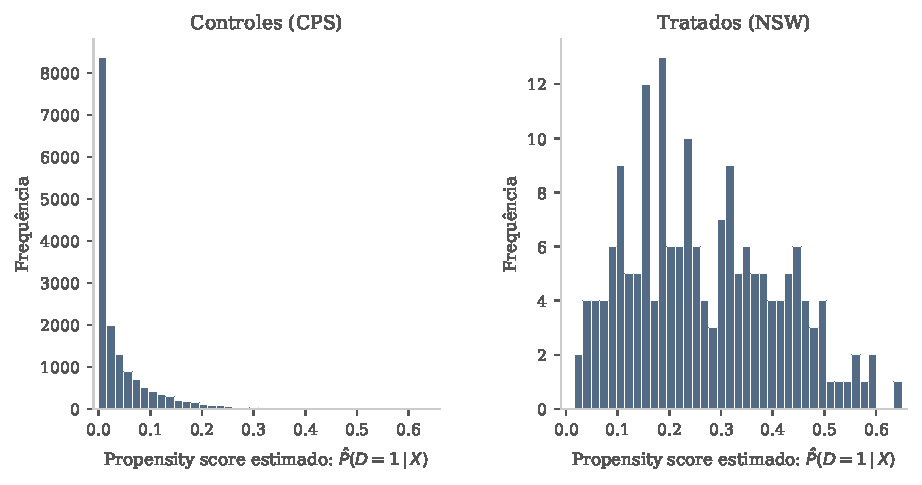
\includegraphics[width=0.9\linewidth]{Figuras/propensity_score.pdf}
    \caption{Distribuição dos \textit{Propensity Scores} estimados para os Controles e Tratados}
    \label{dist}
\end{figure}

\subsubsection{\textit{Nearest-Neighbor} pelo \textit{Propensity Score}}

Uma vez introduzido o \textit{propensity score} como resumo escalar das covariadas, a forma mais natural de usá-lo é simplesmente aplicar nele a mesma lógica de vizinho mais próximo que estudamos antes no caso unidimensional. A ideia é direta: em vez de comparar tratados e controles com base na distância em idade, escolaridade, renda, etc. simultaneamente, passamos a compará-los com base na distância em uma única variável contínua, o $\hat{p}(X_i)$. O problema de pareamento multivariado se transforma, assim, em um problema de pareamento com uma variável só.

No \textit{nearest neighbor} pelo \textit{propensity score}, cada indivíduo tratado é emparelhado com um ou alguns indivíduos de controle cujo \textit{propensity score} seja o mais próximo possível. A noção de “proximidade” aqui é simplesmente a diferença absoluta $|\hat{p}(X_i) - \hat{p}(X_j)|$. Dois indivíduos podem ser muito diferentes em termos de idade e escolaridade, mas se a combinação dessas covariadas leva a uma probabilidade semelhante de tratamento, o método os considera comparáveis do ponto de vista da seleção.

Em termos operacionais, o procedimento pode ser descrito em etapas bastante claras. Primeiro, estima-se o \textit{propensity scor}e $\hat{p}(X_i)$ para toda a amostra. Em seguida, para cada tratado, calcula-se a distância em $\hat{p}(X_i)$ em relação a todos os controles e identifica-se aquele (ou aqueles) que minimizam essa distância. O contrafactual do tratado passa a ser o resultado observado desse(s) controle(s), tal como no vizinho mais próximo com uma variável estudado na Seção 4.

No contexto do NSW, isso significa o seguinte. Em vez de tentar encontrar, para cada participante do programa, um controle que seja simultaneamente parecido em idade, escolaridade, experiência e renda passada, primeiro ajustamos um modelo que explique quem entra ou não entra no programa com base nessas covariadas. Esse modelo nos fornece, para cada indivíduo, uma probabilidade estimada de participação $\hat{p}(X_i)$. Depois, para um jovem tratado com $\hat{p}(X_i) = 0,45$, por exemplo, procuramos no grupo de controle indivíduos cujo $\hat{p}(X_i)$ seja muito próximo de 0,45 — talvez 0,44, 0,46, 0,43. A comparação deixa de ser “quem se parece em todas as características” e passa a ser “quem tinha chances semelhantes de ser selecionado”.

Todas as decisões práticas do pareamento reaparecem aqui, mas agora em um eixo só. Ainda precisamos decidir se vamos usar apenas um controle por tratado ou mais de um. Se optarmos por um único vizinho, o emparelhamento é pontual e muito fácil de interpretar: o tratado é comparado com o controle que tinha probabilidade de tratamento mais parecida com a sua. Se optarmos por dois, três ou mais vizinhos, começamos a construir médias de controles em torno de cada tratado, reduzindo a variância à custa de admitir comparações um pouco menos próximas em $\hat{p}(X_i)$.

Da mesma forma, continua sendo essencial decidir qual é o pior pareamento aceitável. Mesmo em termos de \textit{propensity score}, pode haver tratados em regiões de quase ausência de controles. Por exemplo, indivíduos tratados com $\hat{p}(X_i)$ muito próximo de 1 terão pouquíssimos controles disponíveis na mesma faixa. Na prática, impõe-se um limite máximo para $|\hat{p}(X_i) - \hat{p}(X_j)|$, e tratados que não encontrem controles suficientemente próximos são excluídos da análise. Esse corte explicita a região de suporte comum em termos do \textit{propensity score}: é justamente o intervalo de valores para os quais existem, de fato, tratados e controles.

Em síntese, o \textit{nearest neighbor} pelo \textit{propensity score} combina duas ideias centrais deste capítulo. De um lado, usa o \textit{propensity score} como instrumento de redução de dimensionalidade, transformando um problema de alta dimensão em um problema unidimensional. De outro, aplica nessa dimensão reduzida a lógica já familiar do pareamento por vizinho mais próximo. O resultado é um procedimento que torna viável, na prática, a lógica da CIA em aplicações com muitas covariadas, preservando a transparência da comparação individual entre tratados e controles.

A seguir, iremos estimar tanto o ATE quanto o ATT utilizando vizinhos mais próximo com o \textit{propensity score}. O bloco de código abaixo prepara os dados e estima o propensity score.

\begin{boxH}
\begin{lstlisting}[language = R]

# -----------------------------
# 1) Preparação + estimação do propensity score
# -----------------------------
covs <- c("age", "educ", "black", "hisp", "marr", "nodegree",
          "re74", "re75", "u74", "u75")

vars_needed <- c("treat", "re78", covs)

dat <- cps %>%
  dplyr::select(all_of(vars_needed)) %>%
  tidyr::drop_na() %>%
  mutate(treat = as.integer(treat))

# Logit para propensity score
fml_ps <- as.formula(paste("treat ~", paste(covs, collapse = " + ")))
ps_model <- glm(fml_ps, data = dat, family = binomial("logit"))

dat <- dat %>%
  mutate(pscore = predict(ps_model, type = "response"))

# Vetores para Matching::Match
Y  <- dat$re78
Tr <- dat$treat

# X como matriz N x 1 (propensity score)
Xps <- as.matrix(dat$pscore)

\end{lstlisting}
\end{boxH}

A seguir, iremos construir a função auxiliar \texttt{run\_nn\_ps} para facilitar o cálculo dos resultados.

\begin{boxH}
\begin{lstlisting}[language = R]

# -----------------------------
# 2) Função auxiliar para rodar NN matching no pscore
# -----------------------------
run_nn_ps <- function(M, estimand = c("ATT", "ATE")) {
  estimand <- match.arg(estimand)
  
  out <- Match(
    Y = Y,
    Tr = Tr,
    X = Xps,          # distância é |ps_i - ps_j|
    M = M,
    replace = TRUE,
    estimand = estimand
  )
  
  tibble(
    estimand = estimand,
    M = M,
    estimate = out$est,
    se_AI = out$se,
    t_stat = out$t
  )
}

\end{lstlisting}
\end{boxH}

Por fim, iremos estimar o ATE e o ATT para três valores de vizinhos mais próximos: 1, 3 e 5.

\begin{boxH}
\begin{lstlisting}[language = R]

# -----------------------------
# 3) Rodar M = 1, 3, 5 (ATT e ATE)
# -----------------------------
Ms <- c(1, 3, 5)

results_ps <- bind_rows(
  lapply(Ms, run_nn_ps, estimand = "ATT"),
  lapply(Ms, run_nn_ps, estimand = "ATE")  # remova esta linha se quiser apenas ATT
) %>%
  mutate(est_se = sprintf("%.3f (%.3f)", estimate, se_AI))

print(results_ps)

\end{lstlisting}
\end{boxH}

A Tabela \ref{nnps} apresenta as estimativas obtidas por pareamento de vizinho mais próximo utilizando o \textit{propensity score} como métrica de distância. No Painel A, observa-se que as estimativas do efeito médio sobre os tratados (ATT) são positivas e, em magnitude, mais próximas do efeito estimado a partir dos dados experimentais quando comparadas às estimativas obtidas por métodos ingênuos. Além disso, o ATT mostra relativa estabilidade à escolha do número de vizinhos mais próximos, o que sugere que o \textit{propensity score}, ao resumir a informação das covariadas em uma única dimensão, permite construir um grupo de controle mais comparável aos tratados ao menos nas regiões em que há algum grau de sobreposição. Esses resultados indicam que o pareamento pelo \textit{propensity score} consegue reduzir parte do viés de seleção relevante para a população tratada.

Em contraste, o Painel B evidencia que a estimação do efeito médio do tratamento (ATE) permanece problemática. As estimativas do ATE são negativas, sensíveis à escolha do número de vizinhos mais próximos e distantes do efeito experimental, refletindo a dificuldade de identificar efeitos causais médios em toda a população a partir de dados não experimentais. Como o ATE exige comparações válidas ao longo de toda a distribuição de covariadas, incluindo regiões com baixa probabilidade de tratamento, o pareamento por vizinho mais próximo acaba recorrendo a comparações entre unidades pouco semelhantes, o que introduz extrapolação implícita e viés residual. Assim, mesmo utilizando o \textit{propensity score} como critério de pareamento, o pareamento continua incapaz de recuperar um efeito causal para a população como um todo, ressaltando a importância do suporte comum e os limites do ATE em contextos observacionais.

\begin{table}[htbp]
\centering
\caption{Nearest Neighbor Matching pelo Propensity Score}
\label{tab:nn_pscore_trimmed}
\begin{tabular}{lccc}
\toprule
 & \multicolumn{3}{c}{Número de vizinhos mais próximos ($M$)} \\
\cmidrule(lr){2-4}
 & $1$ & $3$ & $5$ \\
\midrule
\multicolumn{4}{l}{\textbf{Painel A: Efeito Médio sobre os Tratados (ATT)}} \\
\midrule
Tratamento 
& 1322.142 
& 1075.699 
& 1193.554 \\
 
& (943.412) 
& (818.544) 
& (812.322) \\
\midrule
\multicolumn{4}{l}{\textbf{Painel B: Efeito Médio do Tratamento (ATE)}} \\
\midrule
Tratamento 
& -4027.222 
& -7149.183 
& -7009.720 \\
 
& (4238.945) 
& (3389.585) 
& (2771.592) \\
\bottomrule
\end{tabular}

\begin{flushleft}
\footnotesize
\textit{Notas}: A tabela reporta estimativas do efeito médio do tratamento sobre os tratados (ATT) e do efeito médio do tratamento (ATE) obtidas por matching de vizinho mais próximo utilizando o propensity score como métrica de distância. O número de vizinhos mais próximos é indicado por $M$. Os erros-padrão (entre parênteses) seguem a correção analítica de Abadie--Imbens. Todos os pareamentos são realizados com reposição.
\end{flushleft}\label{nnps}
\end{table}


Na subseção seguinte, veremos uma forma alternativa de usar o \textit{propensity score}: em vez de selecionar vizinhos com $\hat{p}(X_i)$ semelhante, vamos utilizar o próprio \textit{propensity score} para construir pesos e formar grupos sintéticos de comparação, por meio de métodos de ponderação.

\subsubsection{Ponderação pelo \textit{Propensity Score}}

Na subseção anterior, utilizamos o \textit{propensity score} para selecionar comparações locais, emparelhando cada tratado com controles de propensão semelhante. Há, porém, uma segunda forma — igualmente natural e muito poderosa — de explorar a propriedade de balanceamento do \textit{propensity score}: em vez de selecionar vizinhos, podemos utilizá-lo diretamente para construir pesos, formando grupos sintéticos de comparação. Essa abordagem é conhecida como ponderação pelo \textit{propensity score}.

A lógica econômica da ponderação é a seguinte. Se indivíduos com diferentes probabilidades de tratamento estão desproporcionalmente representados nos grupos de tratados e controles, podemos reponderar as observações de modo que, após a ponderação, a composição dos grupos se torne comparável. Em vez de “escolher” explicitamente quem será comparado com quem, o método ajusta automaticamente o peso de cada observação para corrigir o viés de seleção observável.

Sob a Hipótese de Independência Condicional, a identificação do efeito causal depende apenas de tornar a seleção no tratamento independente dos resultados potenciais. Como vimos na Seção 5.2, essa independência é garantida ao condicionarmos no \textit{propensity score}. A ponderação faz isso não por meio de condicionamento direto, mas por meio da reconstrução artificial da distribuição das covariadas.

Considere, por exemplo, um indivíduo com probabilidade muito baixa de participar do programa, digamos $\hat{p}(X_i) = 0,1$. Se ele aparece no grupo tratado, esse tipo de indivíduo é “raro” entre os tratados e deve receber peso pequeno. Já no grupo de controle, esse tipo de indivíduo é muito comum e, portanto, deve receber peso elevado. O oposto ocorre para indivíduos com \textit{propensity score} alto. Assim, a ponderação usa exatamente a escassez ou abundância relativa de cada perfil para corrigir o viés de composição.

O resultado desse processo é a construção de uma pseudo-população na qual, por construção, a distribuição das covariadas é a mesma entre tratados e controles. Nessa pseudo-população, a alocação do tratamento é, no sentido observável, tão boa quanto aleatória. O estimador por ponderação mais básico é o chamado \textit{Inverse Probability Weighting} (IPW). Quando o objetivo é identificar o ATE, o estimador ponderado é dado por
$$
\widehat{ATE}_{IPW} = \frac{1}{N} \sum_{i=1}^{N}\left(\frac{D_i Y_i}{\hat{p}(X_i)} - \frac{1- D_iY_i}{1-\hat{p}(X_i)}\right)
$$

A interpretação dessa expressão é direta. Cada resultado observado dos tratados é inflado pelo inverso da sua probabilidade de tratamento, enquanto cada resultado observado dos controles é inflado pelo inverso da sua probabilidade de não tratamento. Observações que eram improváveis de estar no grupo em que de fato estão recebem peso maior.

Quando o objetivo é o Efeito Médio sobre os Tratados (ATT), a ponderação muda apenas no grupo de controle. O estimador passa a ser

$$
\widehat{ATT}_{IPW} = \frac{1}{N_1} \sum_{i : D_i = 1} Y_i - \frac{1}{N_1} \sum_{i : D_i = 0} \frac{\hat{p}(X_i)}{1-\hat{p}(X_i)}Y_i,
$$

\noindent onde $N_1$ é o número de tratados. esse caso, os tratados entram com peso unitário, e os controles são reponderados para reproduzir a distribuição dos tratados em termos de \textit{propensity score.
}
Do ponto de vista conceitual, esse segundo termo corresponde exatamente ao contrafactual médio dos tratados, construído como uma média ponderada dos resultados dos controles, em que os pesos dependem da razão $\frac{\hat{p}(X_i)}{1-\hat{p}(X_i)}$.

Abaixo, iremos estimar o ATE e o ATT através dos estimadores de IPW. No bloco de código a seguir, iremos preparar as variáveis e calcular o \textit{propensity score}.

\begin{boxH}
\begin{lstlisting}[language = R]
# -----------------------------
# 1) Preparação + propensity score
# -----------------------------
covs <- c("age", "educ", "black", "hisp", "marr", "nodegree",
          "re74", "re75", "u74", "u75")

vars_needed <- c("treat", "re78", covs)

dat <- cps %>%
  dplyr::select(all_of(vars_needed)) %>%
  tidyr::drop_na() %>%
  mutate(treat = as.integer(treat))

fml_ps <- as.formula(paste("treat ~", paste(covs, collapse = " + ")))
ps_model <- glm(fml_ps, data = dat, family = binomial("logit"))

dat <- dat %>%
  mutate(pscore = predict(ps_model, type = "response"))

\end{lstlisting}
\end{boxH}

A seguir, iremos limitar nossa amostra para valores do \textit{propensity score} acima de 0,1 e abaixo de 0,9. Isso nos ajuda a evitar pesos extremos, que podem alterar nosso resultado de forma substancial.

\begin{boxH}
\begin{lstlisting}[language = R]
# -----------------------------
# 2) Trimming (recomendado)
# -----------------------------
dat <- dat %>%
  filter(!(pscore >= 0.9)) %>% 
  filter(!(pscore <= 0.1))

\end{lstlisting}
\end{boxH}

No bloco de código abaixo iremos calcular os pesos referentes aos estimadores de IPW do ATE e do ATT.

\begin{boxH}
\begin{lstlisting}[language = R]


# -----------------------------
# 3) IPW weights (ATE e ATT)
# -----------------------------

dat <- dat %>%
  mutate(
    # Pesos brutos
    w_ate = treat/pscore + (1 - treat)/(1 - pscore),
    
    w_att = ifelse(treat == 1, 1, pscore/(1 - pscore))
  ) 

\end{lstlisting}
\end{boxH}

Por fim, iremos estimar o ATE e o ATT usando os pesos construídos no bloco acima.

\begin{boxH}
\begin{lstlisting}[language = R]
# -----------------------------
# 4) Estimativas IPW (ATE e ATT)
# -----------------------------


fit_ate <- lm_robust(re78 ~ treat, data = dat, weights = w_ate)

fit_att <- lm_robust(re78 ~ treat, data = dat, weights = w_att)

summary(fit_ate)
summary(fit_att)

\end{lstlisting}
\end{boxH}

A Tabela \ref{ipw} apresenta as estimativas obtidas por ponderação inversa da probabilidade de tratamento (IPW). Diferentemente dos resultados baseados em regressões simples e em pareamento por vizinho mais próximo, o IPW produz estimativas tanto do efeito médio do tratamento (ATE) quanto do efeito médio sobre os tratados (ATT) que se aproximam substancialmente do efeito estimado a partir dos dados experimentais. Em particular, o ATT estimado é positivo, estatisticamente significativo e de magnitude muito semelhante àquela obtida no experimento, indicando que a reponderação das observações do grupo de controle consegue reproduzir de forma mais adequada o contrafactual relevante para os indivíduos tratados.

Além disso, o IPW também apresenta um desempenho superior na estimação do ATE, cujo valor estimado é positivo e consideravelmente mais próximo do efeito experimental quando comparado às estimativas obtidas por pareamento. Esse resultado sugere que, ao explorar de maneira contínua a informação contida no \textit{propensity score} e utilizar toda a amostra disponível por meio de pesos, o IPW reduz a necessidade de extrapolações extremas implícitas nos métodos de pareamento por vizinhos mais próximos. Ainda que a validade dessas estimativas dependa fortemente da correta especificação do \textit{propensity score} e da existência de suporte comum, os resultados da tabela indicam que a ponderação inversa constitui uma abordagem mais eficaz para recuperar efeitos causais médios em dados não-experimentais, especialmente quando o objetivo é aproximar tanto o ATT quanto o ATE do benchmark experimental.


\begin{table}[h]
\centering
\caption{Resultados do IPW}
\begin{talltblr}[         %% tabularray outer open
entry=none,label=none,
note{}={+ p \num{< 0.1}, * p \num{< 0.05}, ** p \num{< 0.01}, *** p \num{< 0.001}},
]                     %% tabularray outer close
{                     %% tabularray inner open
colspec={Q[]Q[]Q[]},
column{2-3}={}{halign=c,},
column{1}={}{halign=l,},
hline{4}={1-3}{solid, black, 0.05em},
}                     %% tabularray inner close
\toprule
& ATE & ATT \\ \midrule %% TinyTableHeader
Tratamento \hspace{80mm} & \num{1533.798}+ & \num{2056.846}** \\
& (\num{807.560}) & (\num{775.559}) \\
Num.Obs. & \num{452} & \num{452} \\
\bottomrule
\end{talltblr}\label{ipw}
\end{table} 

Um aspecto crucial da ponderação é que ela é particularmente sensível a problemas de suporte comum. Se houver indivíduos com $\hat{p}(X_i)$ muito próximo de 0 ou de 1, os pesos $1/\hat{p}(X_i)$ ou $1/(1-\hat{p}(X_i))$ tornam-se extremamente elevados, fazendo com que poucas observações dominem o estimador. Por esse motivo, na prática, é comum aplicar cortes no \textit{propensity score}, excluindo observações com valores extremos, ou truncar os pesos.

Esse problema é menos agudo no \textit{nearest neighbor}, que simplesmente descarta tratados sem bons controles. Na ponderação, por outro lado, indivíduos mal suportados permanecem na amostra, mas entram com pesos desproporcionalmente grandes, o que pode aumentar drasticamente a variância e gerar instabilidade.

As duas abordagens exploram a mesma base teórica — o \textit{propensity score} como estatística de balanceamento sob a CIA —, mas o fazem de maneiras complementares. O \textit{nearest neighbor} constrói o contrafactual individual de cada tratado por meio de comparações locais. A ponderação constrói o contrafactual médio por meio de uma transformação global da amostra.

No contexto do NSW, isso significa que, em vez de procurar, para cada participante do programa, um controle com probabilidade semelhante de participação, podemos utilizar todos os controles disponíveis, atribuindo pesos maiores àqueles cujo perfil os torne mais parecidos com os tratados em termos de seleção observável. Ambas as estratégias buscam o mesmo objetivo: reproduzir, com dados observacionais, a lógica de um experimento aleatório.

\subsection{Notas sobre Inferência}

Ao longo deste guia, adotamos procedimentos de inferência que refletem a prática empírica padrão para métodos de matching e ponderação, mas é importante deixar explícito que a inferência nesses contextos envolve sutilezas técnicas relevantes. Diferentemente de regressões lineares usuais, os estimadores baseados em matching e em propensity score dependem de objetos estimados em uma primeira etapa, o que altera sua distribuição amostral e torna inadequada a aplicação direta de fórmulas clássicas de variância.

No caso do nearest neighbor matching, a inferência é particularmente delicada devido à não suavidade do estimador e à reutilização de observações do grupo de controle. Por esse motivo, utilizamos a correção analítica proposta por Abadie e Imbens, que ajusta os erros-padrão levando explicitamente em conta a estrutura do pareamento. Essa abordagem constitui a referência padrão na literatura para inferência em matching por vizinho mais próximo.

No caso da ponderação pelo propensity score (IPW), a inferência prática costuma ser realizada por meio de erros-padrão robustos obtidos a partir de regressões ponderadas. Esse procedimento trata o propensity score estimado como conhecido e, portanto, não incorpora explicitamente a incerteza da primeira etapa. Sob condições regulares — como modelos bem especificados e amostras moderadas — essa aproximação tende a funcionar razoavelmente bem e é amplamente utilizada em aplicações empíricas. Ainda assim, ela não é plenamente eficiente do ponto de vista assintótico geral.

A literatura recente tem enfatizado métodos de inferência mais rigorosos baseados em funções de influência e em estimadores doubly robust, como o AIPW e o TMLE, que permitem incorporar automaticamente a incerteza da estimação do propensity score e de modelos auxiliares. Esses métodos representam o estado da arte em inferência causal com dados observacionais, mas exigem ferramentas conceituais e computacionais mais avançadas, que fogem do escopo introdutório deste guia.

Para leitores interessados em aprofundar-se nesses temas, as seguintes referências são particularmente recomendadas:


\begin{itemize}
    \item Abadie e Imbens (2006, 2008), para fundamentos teóricos e inferência em matching por vizinho mais próximo;

\item Hirano, Imbens e Ridder (2003), para resultados assintóticos em estimadores baseados em propensity score;

\item van der Laan e Rose (2011), para inferência via TMLE;

\item Chernozhukov et al. (2018), para estimadores doubly robust com cross-fitting e aprendizado de máquina.
\end{itemize}

Em síntese, os métodos apresentados neste guia fornecem inferência adequada para aplicações empíricas padrão, ao mesmo tempo em que abrem caminho para abordagens mais sofisticadas quando maior rigor inferencial é necessário.


%\section{\sc Pareamento em Outros Métodos}\label{multihip}

%\input{Sections/6 - Policymakers}

\section{\sc Conclusão}

\input{Sections/8 - Conclusão}

\setlength\bibsep{0pt}
\bibliographystyle{mystyle} 
\bibliography{ref.bib}


\end{document}

